\section{A Route to Visualisation} \label{sec:visualisation}


\subsection{Initial reductions}


    As the points in our state space are six-dimensional vectors of the form of \cref{eq:stateVector},
    % \begin{equation*}
    %     \boldsymbol{x}
    %     =
    %     \begin{pmatrix}
    %     \boldsymbol{r} \\
    %     \boldsymbol{v}
    %     \end{pmatrix}
    %     =
    %     \begin{pmatrix}
    %     x \\ y \\ z \\ v_x \\ v_y \\ v_z
    %     \end{pmatrix},
    % \end{equation*}
    we first apply several considerations to make our investigations more manageable.

    The first of these is the least restrictive: As noted in \cref{sec:CR3BP}, the dynamics of the CR3BP are such that the $z$ and $v_z$ components of a point in our state space may be taken to be $0$. As such, up to isomorphism/omission of these constantly zero indices, we may think of our space as a subset of $\R^4$, giving the first step in our reduction. Informally, we may think of this as the identification
    \begin{equation*}
        % (x,y,0,v_x,v_y,0) \to (x,y,v_x,v_y).
        (x,y,0,v_x,v_y,0) \cong (x,y,v_x,v_y).
    \end{equation*}
%%
%%
    Following this, we face the difficulty of simplifying the dynamics of our system with our desire to more easily analyse it. Towards a compromise in this matter, we employ the use of a Poincaré map, giving the cross-section of trajectories in our state space, with the $y=0$ hyperplane. As is well-established (and known from class), such a use of a Poincaré map still allows us to meaningfully consider the dynamics of a system, while also reducing the dimensionality. In our case, this process results in bringing the above four-dimensional set-up to a more manageable three dimensions. Again, informally this is described by
    \begin{equation*}
        % (x,y,v_x,v_y) \to (x,0,v_x,v_y) \to (x,v_x,v_y).
        (x,y,v_x,v_y) \to (x,0,v_x,v_y) \cong (x,v_x,v_y).
    \end{equation*}
%%
%%
%%
    Finally, when visualisation of our system is particularly important, we may further reduce our space to a two-dimensional set-up via the projection down to the $x,v_y$ plane. Similar as above, this is thought of as
    \begin{equation*}
         (x,v_x,v_y) \to (x,v_x).
    \end{equation*}
    

    The entirety of this reduction is summed up in the following figure:
    \begin{figure}[ht]
        \centering
        
        \begin{tikzpicture}[
            >=Stealth,
            every node/.style={font=\Large}
        ]
        
        % Main spaces
        \node (R6) at (0,0) {$\mathbb{R}^6$};
        \node (R4) at (4,0) {$\mathbb{R}^4$};
        \node (R3) at (8,0) {$\mathbb{R}^3$};
        \node (R2) at (12,0) {$\mathbb{R}^2$};
        
        % Horizontal arrows
        \draw[->, thick] (R6) -- (R4);
        \draw[->, thick] (R4) -- (R3);
        \draw[->, thick] (R3) -- (R2);
        
        % Labels directly above arrows
        \node[font=\normalsize, align=center] at (2,0.6)
        {By CR3BP\\$z=v_z=0$};
        
        \node[font=\normalsize, align=center] at (6,0.6)
        {By Poincaré map\\$y=0$};
        
        \node[font=\normalsize, align=center] at (10,0.6)
        {By projecting to\\$x,v_y$ plane};
        
        % % Small vertical arrow from bottom label to middle arrow
        % \draw[->, thick] (6,-1.0) -- (6,-0.1);
        
        \end{tikzpicture}
        
        \caption{Reduction of the state space dimension.}
    \end{figure}












    \subsection{Constant energy regions} \label{subsec: constant energy regions}

    As alluded to at the end of \cref{sec:CR3BP}, it follows from \cite{KoonLoMarsdenRoss2022} that for a general point of the form $(x,y,v_x,v_y) \in \R^4$, the energy thereof is given by the equation
    %%
    % For a general point of the form $(x,y,v_x,v_y) \in \R^4$, the energy thereof is given by the equation
    \begin{equation} \label{eq:energy}
    	E = \frac{1}{2} \bigl( v_x^2 + v_y^2 \bigr) + \tilde U(x,y),
    \end{equation}
    where $\tilde U(x,y)$ is the augmented potential of the CR3BP,
    \begin{equation}
        \tilde U(x,y) = -\frac{1}{2}(x^2 + y^2) - \frac{\mu_1}{\sqrt{(x+\mu_2)^2 + y^2}} - \frac{\mu_2}{\sqrt{(x-\mu_1)^2 + y^2}} -\frac{1}{2} \mu_1 \mu_2.
    \end{equation}


    
    With the restriction $y=0$ in place from our Poincaré section (the second step in our above reduction), and for a given energy value $E$, it immediately follows from a rearrangement of \cref{eq:energy} that all admissible points $(x,0,v_x,v_y)$ with this energy value are defined by the surface
    \begin{equation} \label{eq:ConstantEnergySurface}
        % v_x^2 + v_y^2 = 2\bigl( E + \tilde U(x,y) \bigr).
        v_x^2 + v_y^2 = 2\bigl( E + \tilde U(x,0) \bigr).
    \end{equation}
    We therefore refer to these surfaces as \textit{surfaces of constant energy}.
    % For obvious reasons, we refer to these surfaces as \textit{surfaces of constant energy}.



    

    % % One particular such surface is that corresponding to the 
    % One particular such surface is that which corresponds to the energy level
    One particular such surface is that defined by
    $$
        % E_2 = \textcolor{red}{\textbf{WHAT IS THE VALUE (AND UNITS) FOR THE ENERGY AT L2????}},
        E_2 \approx -1.592,
    $$
    the energy value (in dimensionless CR3BP units) corresponding to the Lagrange point $L_2$. We refer to the region enclosed by this surface as the \textit{accessible region}, as it comprises all states of the form $(x,0,v_x,v_y)$ that have an energy level at or below $E_2$. 
    % As orbiting bodies with energies above that level may leave the Earth-Moon system, this informs the cut-off of the 
    As orbiting bodies with energies above this level may leave the Earth-Moon system, this defines the boundary of the scope of our current work.


    
    % As seen in \cref{fig:accesible region 3D and 2D}, the $3$D plot of the accessible region has two distinct nodes, each roughly shaped like a pseudosphere. The larger of these corresponds to the region around Earth, and the smaller corresponds to that of the Moon.

    As seen in \cref{fig:accesible region 3D and 2D}, the plot of the accessible region has two distinct nodes, each roughly shaped like a pseudosphere. The larger of these corresponds to the region around Earth, and the smaller corresponds to that around the Moon.

    


    

    % Prior to projecting these surfaces down to the $x,v_y$ plane, three-dimensional visualisation 


    % Prior to projecting 



















    
    % \begin{figure}[tb] \label{fig:accesible region 3D and 2D}
    % 	\centering
    %     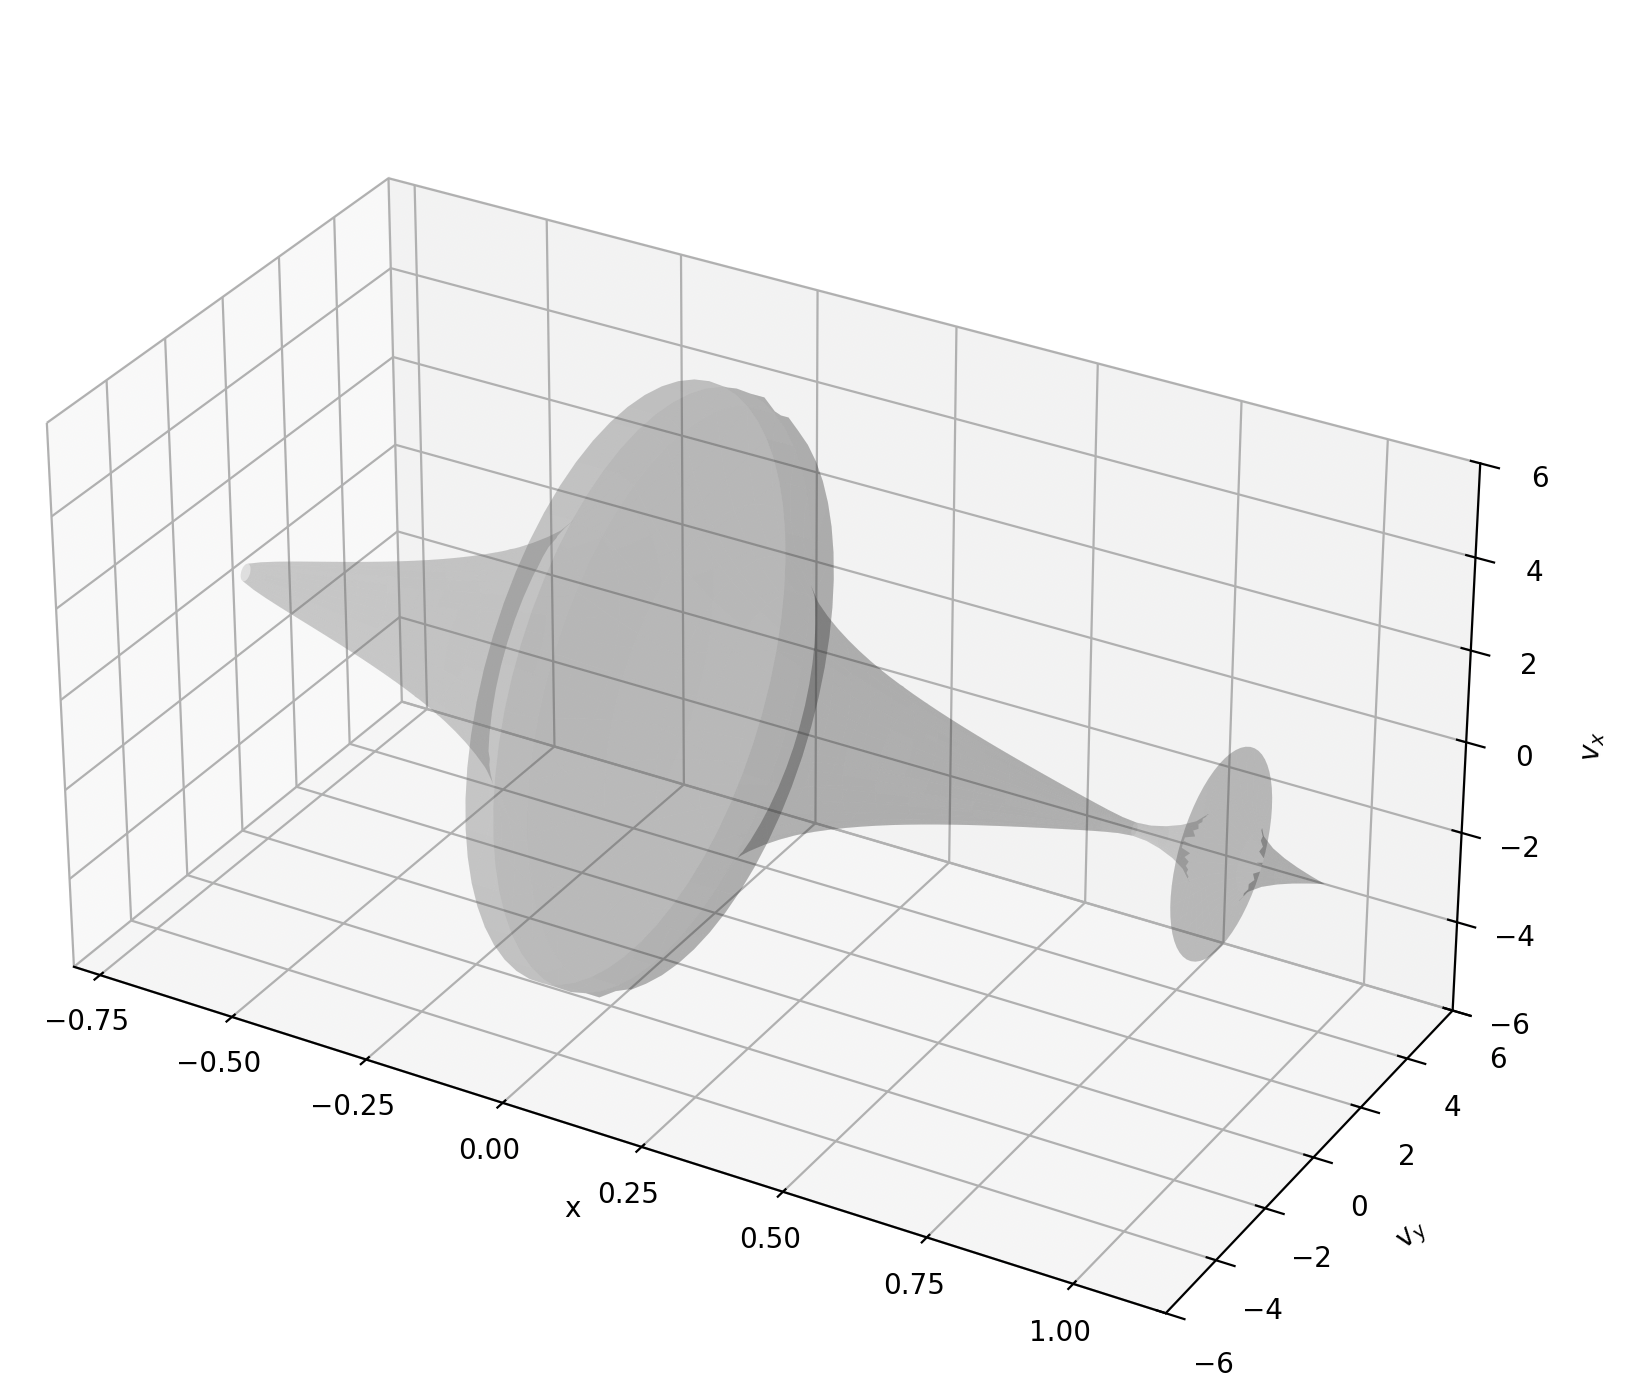
\includegraphics[width=3.1in]{images/Accessible Region 3D.png}
    %     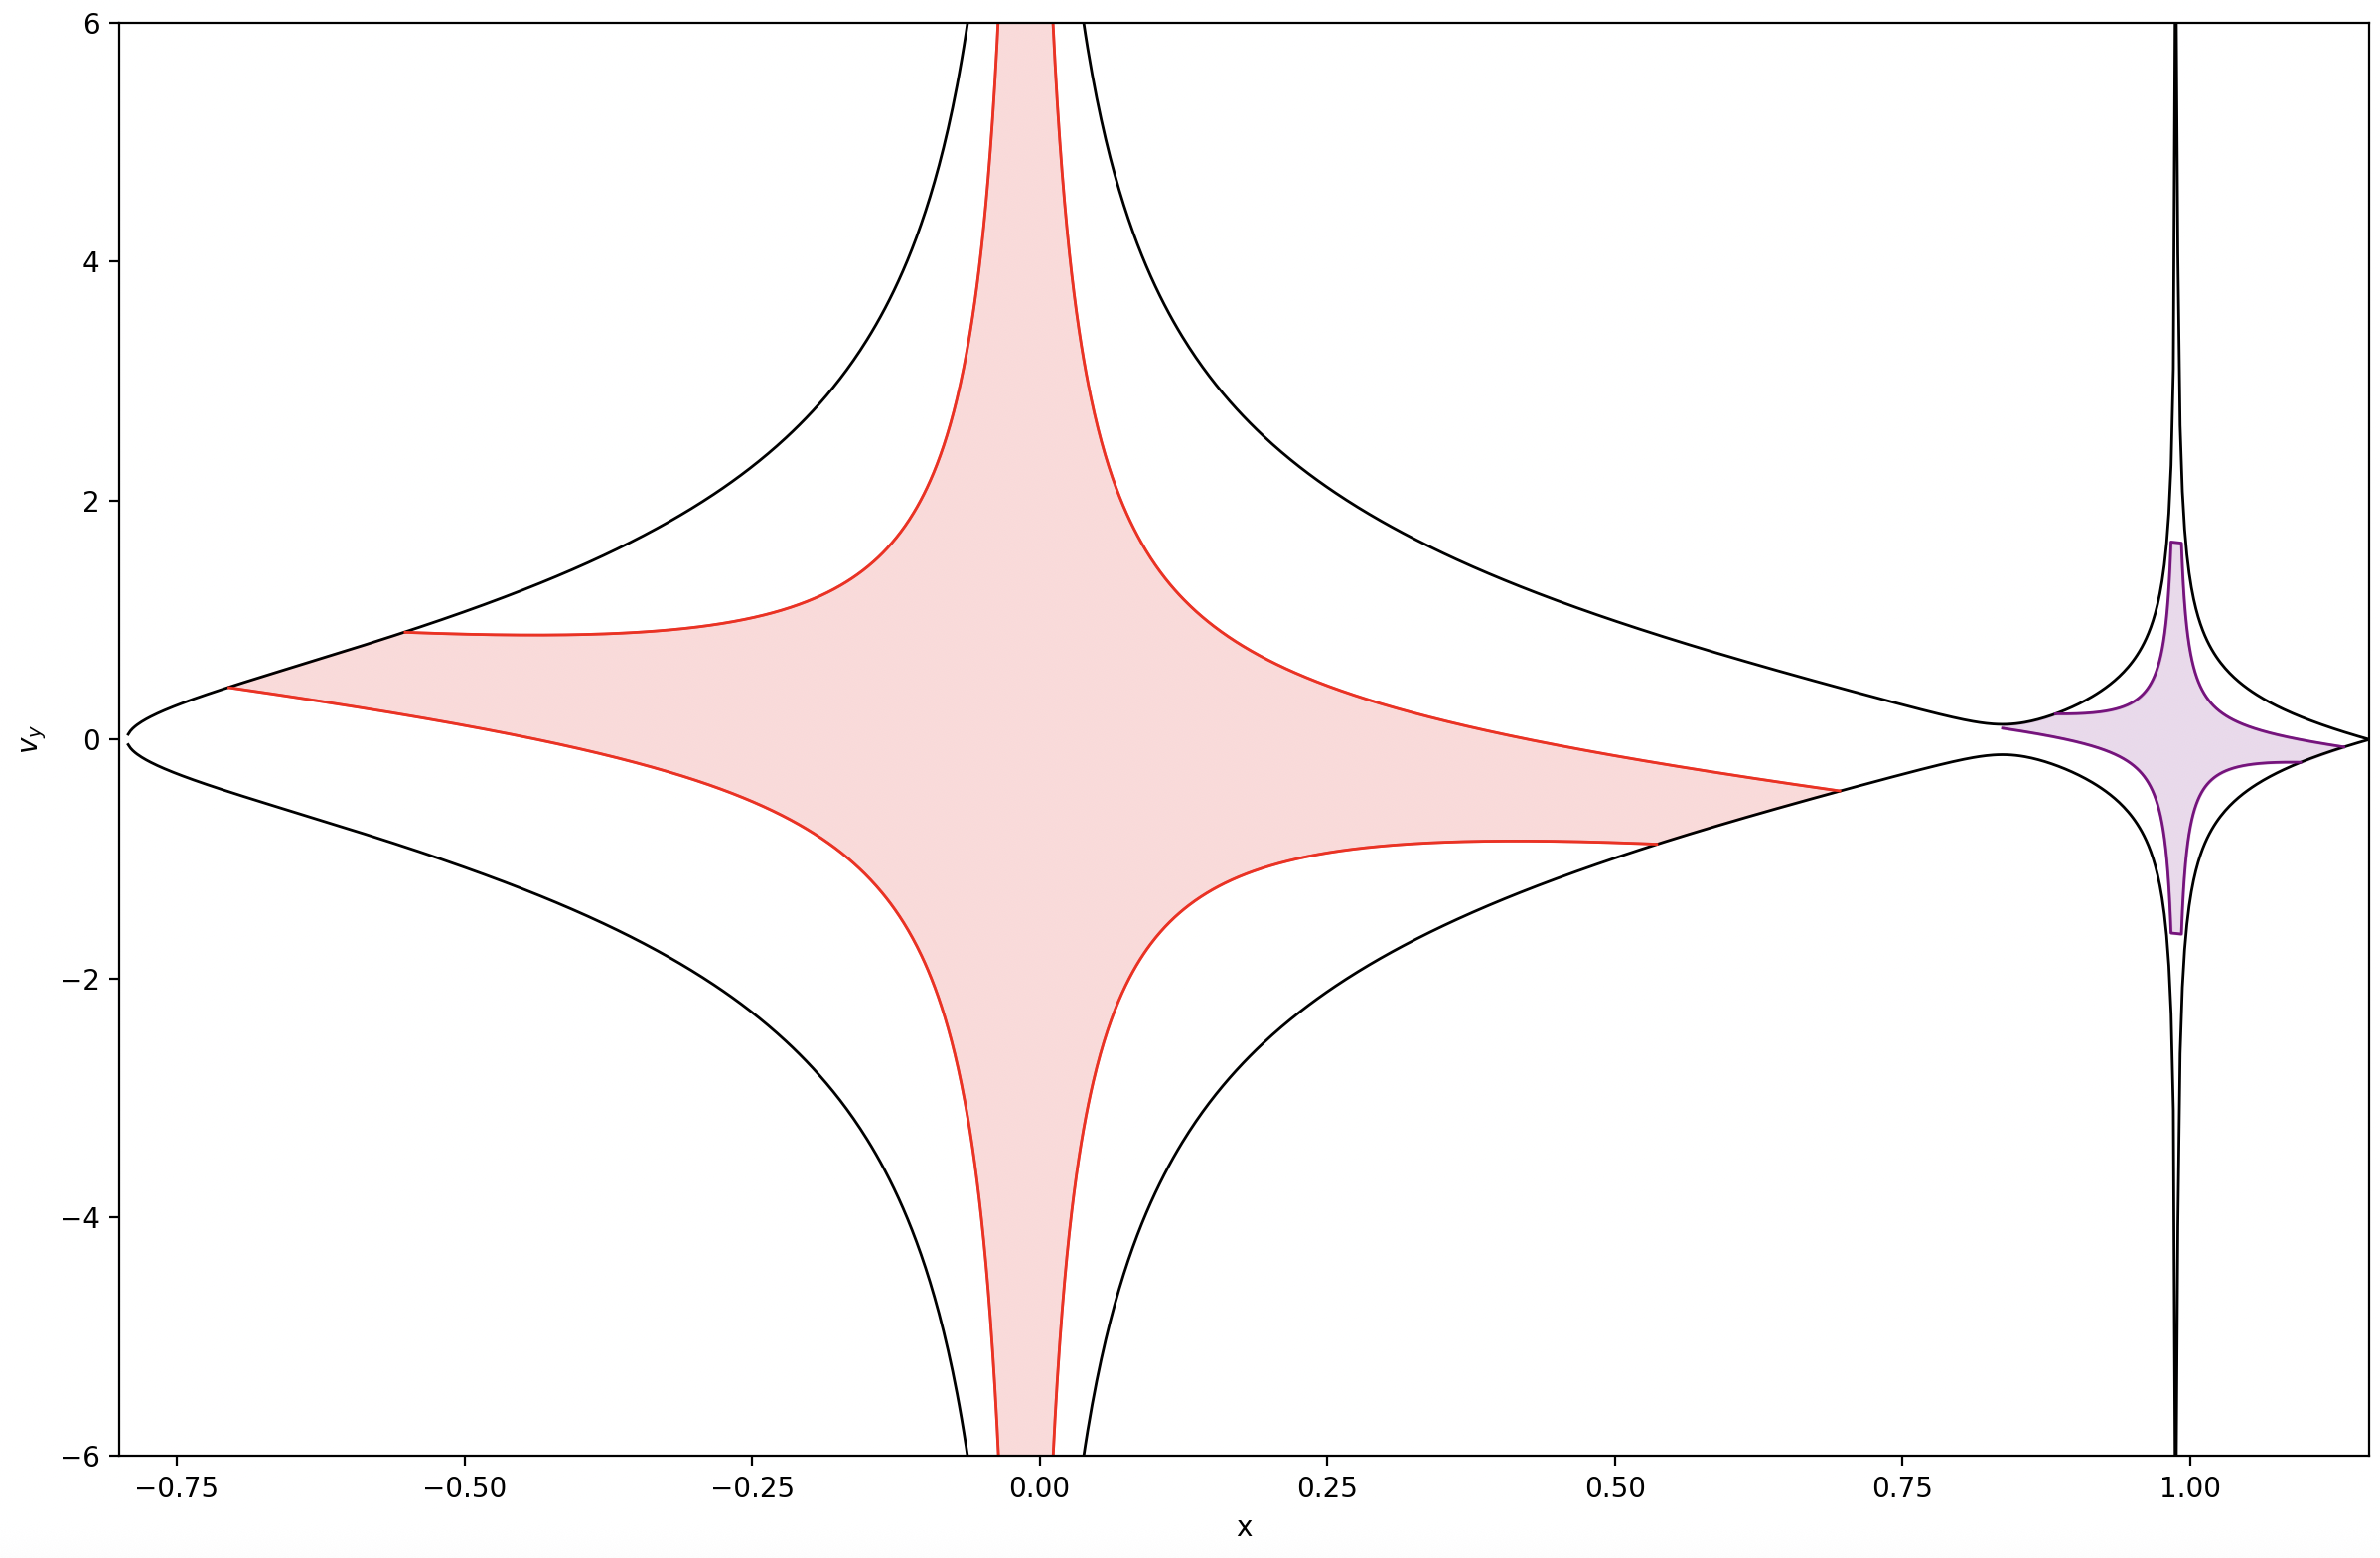
\includegraphics[width=3.2in]{images/2D accessible region with crash regions.png}
    %     \caption{Visualisations of the accessible region in three dimensions and its projection to the $(x,v_y)$ plane, displaying the Earth and Moon crash regions.}
    % \end{figure}

    
    \begin{figure}[tb]
    	\centering
        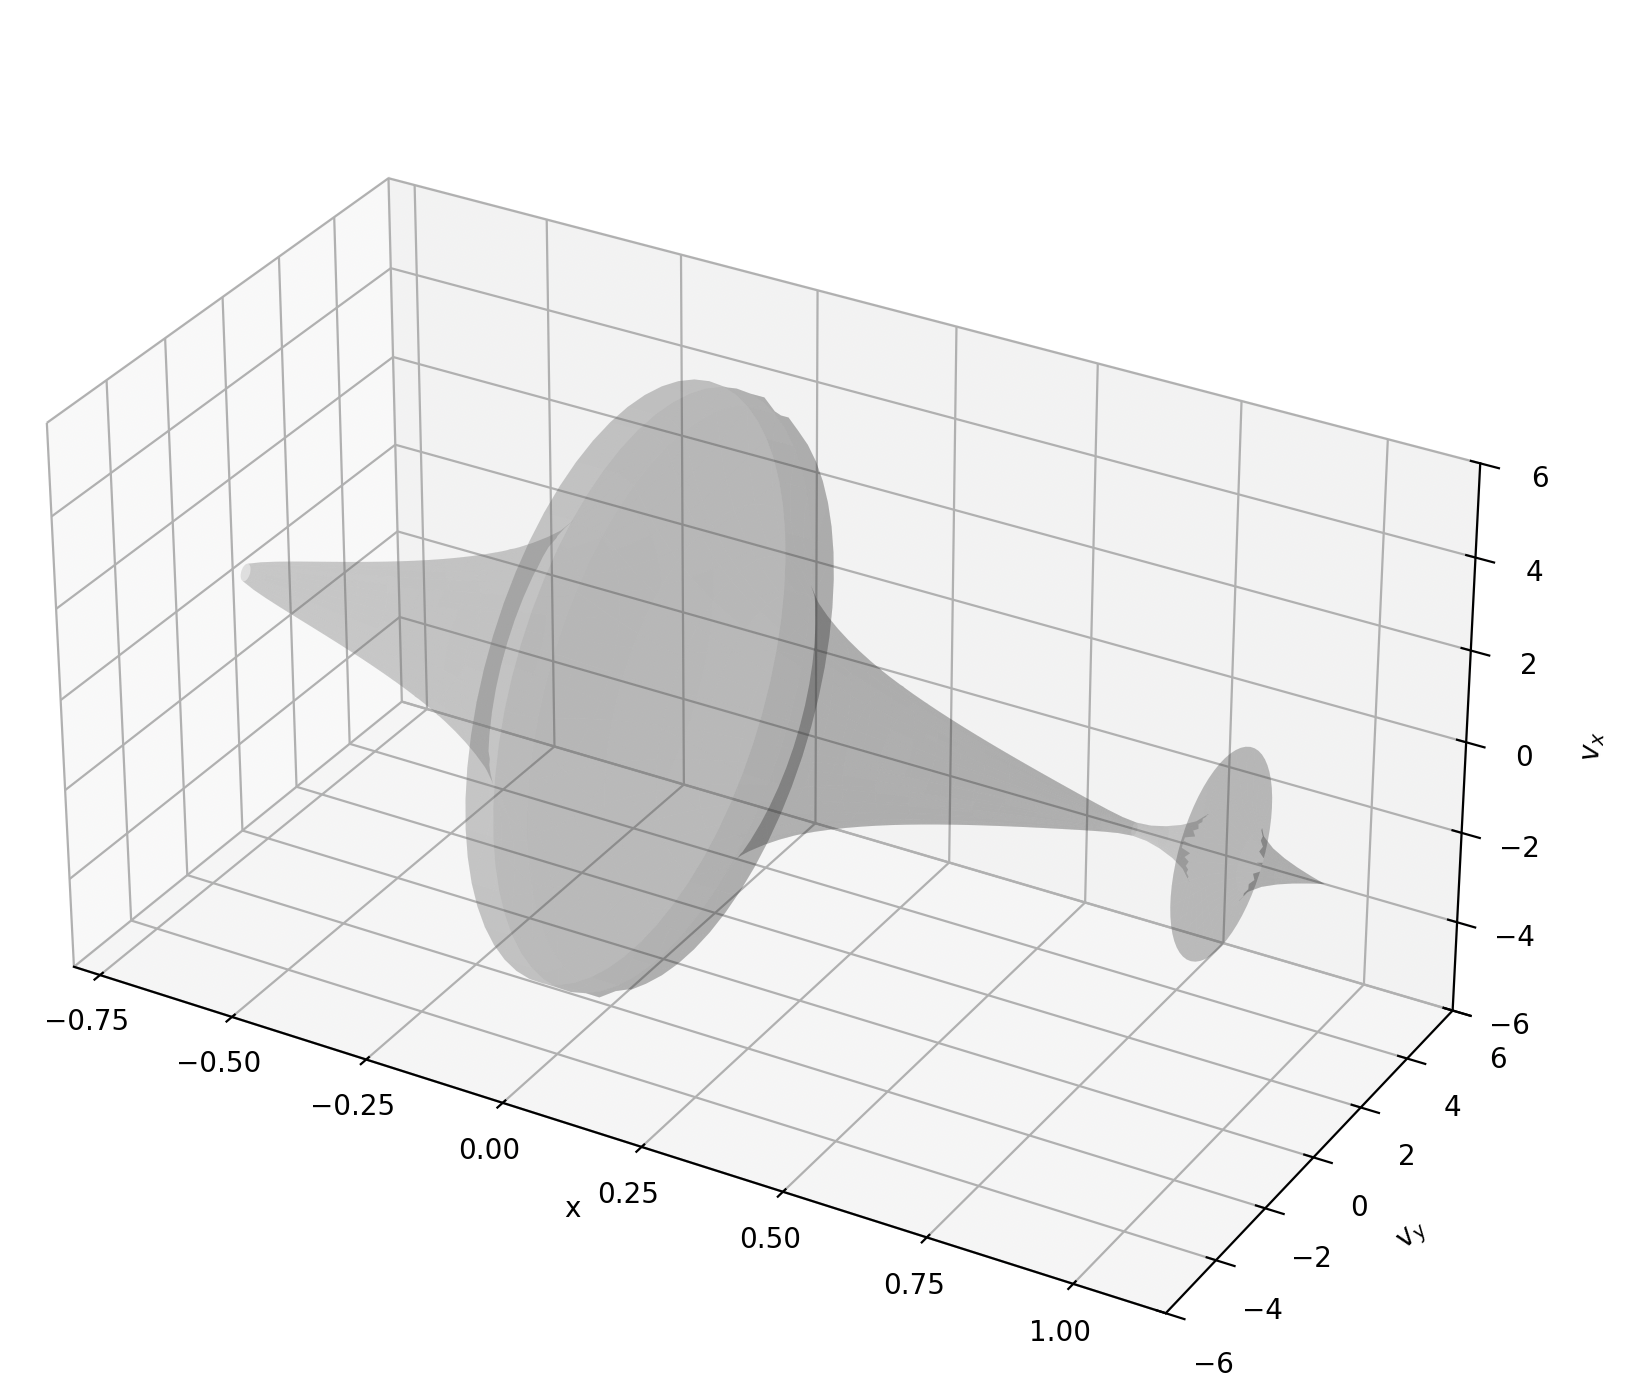
\includegraphics[width=3.1in]{images/Accessible Region 3D.png}
        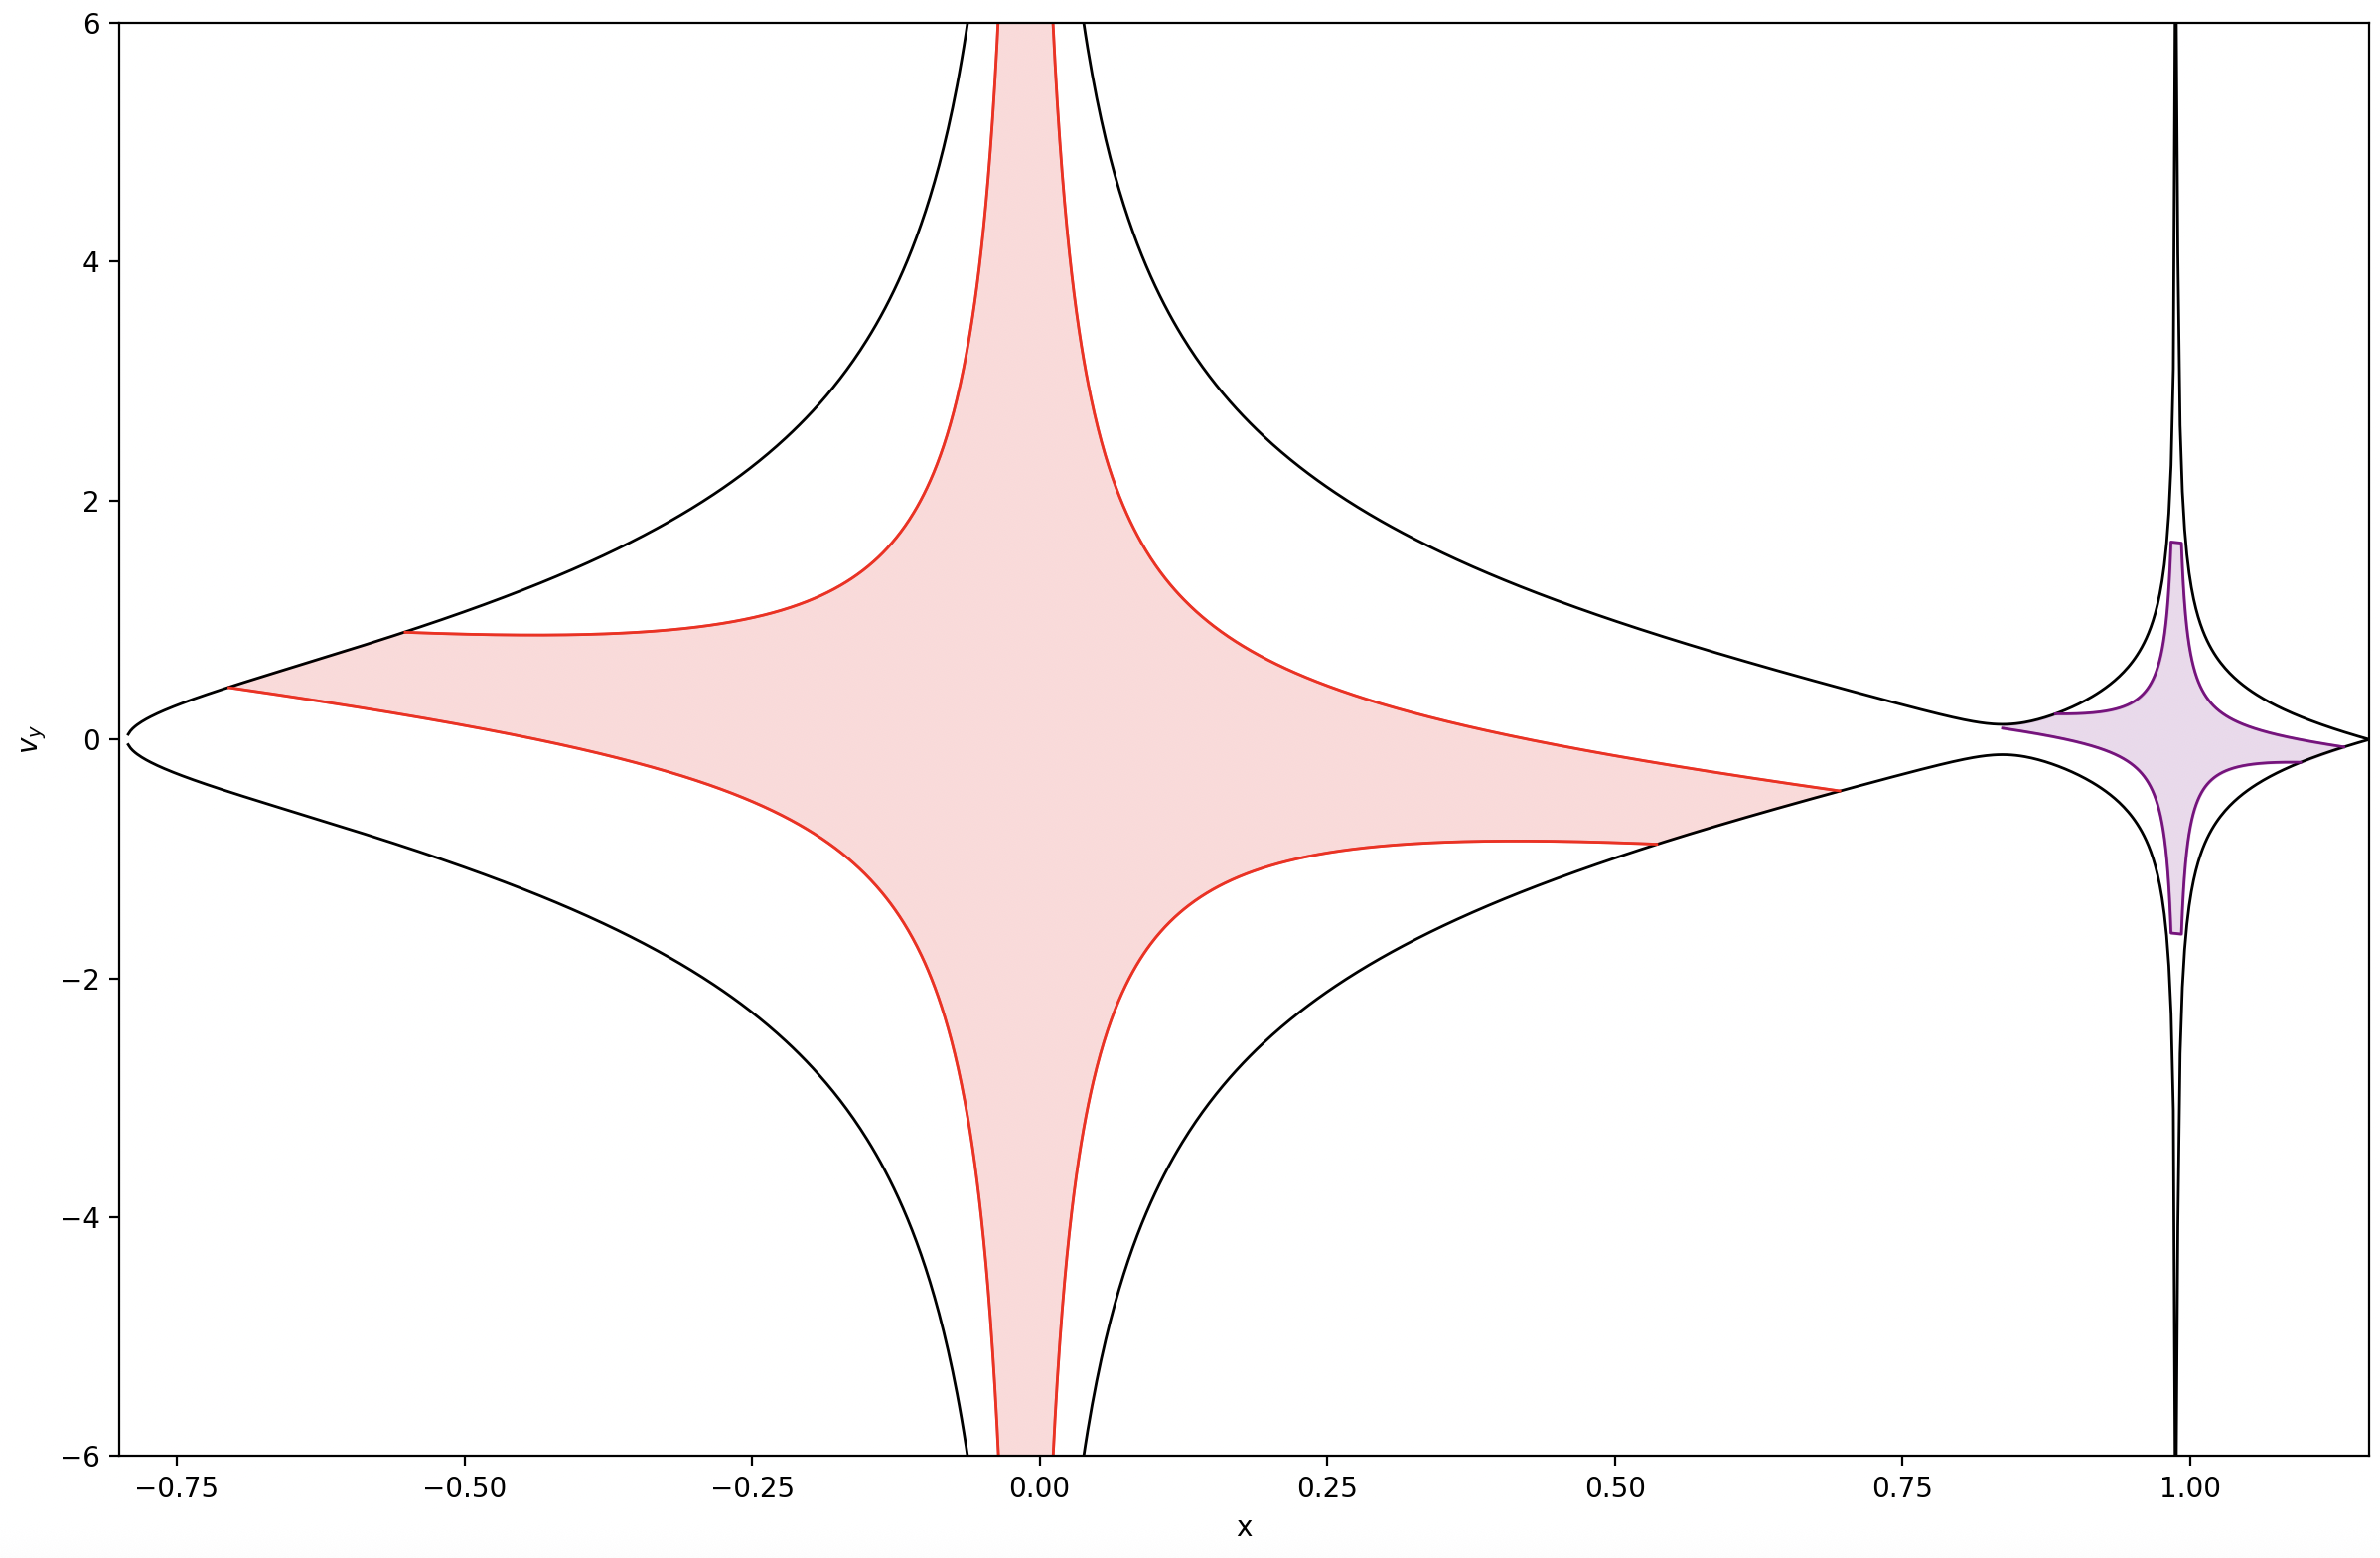
\includegraphics[width=3.2in]{images/2D accessible region with crash regions.png}
        \caption{Visualisations of the accessible region in three dimensions and its projection to the $(x,v_y)$ plane, displaying the Earth and Moon crash regions in red and purple, respectively.}
        \label{fig:accesible region 3D and 2D}
    \end{figure}








    \subsection{The crash region}



    % For certain initial conditions, an orbiting body may quickly enter Earth's atmosphere or crash into the lunar surface. From a practical perspective, points in the state space corresponding to the initial values of such orbits

    % % For certain initial conditions, an orbiting body may quickly enter Earth's atmosphere or crash into the lunar surface. From a practical perspective, points in the state space that will lead to such outcomes when taken as initial conditions are not very interesting, as our object will quickly de-orbit under them.



    For certain initial conditions, an orbiting body may quickly enter Earth's atmosphere or crash into the lunar surface. From a practical perspective, points in the state space leading to these outcomes are not very interesting (or at least, need little consideration), as an object will quickly de-orbit when placed under initial conditions corresponding to them.



    % Arbitrarily, we categorise all points leading to these results within \textit{one} orbital period 





%     We construct a set consisting of all points that will lead to such results within a single orbital period, and refer to it as the \textit{crash region}. The choice of a \textit{single} orbital period is arbitrary, but is chosen due to its convention in relevant literature.
% %
%     Indeed, in the two-dimensionally projected case, this region is analytically derived in \cite{Abraham_Marsden_1987} as the area bounded by the curve
%     \vspace{-0.4cm}
%     \begin{equation} \label{eq:crashRegion}
%     	(v_y + x)^2 =  \frac{R_i^2 v_x^2 + 2 \mu_i R_i \Bigl( 1 - \frac{R_i}{|x-x_i|}\Bigr)}{|x-x_i|^2 - R_i^2},
%     \end{equation}
%      where $\mu_1 = 1-\mu$, $\mu_2 = \mu$ are defined in terms of the normalized mass ratio, \cref{eq:mass ratio}, of the Earth and Moon, $R_1 \approx 7000$, $R_2 = 1738.1$ are the radii of the Earth (including significant portions of the atmosphere) and Moon in kilometres, and $x_1, x_2$ are the distances of the Earth/Moon from the system barycentre, respectively. The Earth and Moon crash regions can both be seen in \cref{fig:accesible region 3D and 2D}.
    



    % We construct a set consisting of all points that will lead to such results within a single orbital period, and refer to it as the \textit{crash region}. The choice of a \textit{single} orbital period is arbitrary, but is chosen due to its convention in relevant literature.
    We construct a set consisting of all points that will lead to such results, and refer to it as the \textit{crash region}.
%
    Indeed, in the two-dimensionally projected case, this region is analytically derived in \cite{Graebner2025}, using techniques from \cite{Abraham_Marsden_1987}, as the area bounded by the curve
    \vspace{-0cm}
    \begin{equation} \label{eq:crashRegion}
    	(v_y + x)^2 =  \frac{R_i^2 v_x^2 + 2 \mu_i R_i \Bigl( 1 - \frac{R_i}{|x-x_i|}\Bigr)}{|x-x_i|^2 - R_i^2},
    \end{equation}
     where $\mu_1 = 1-\mu$, $\mu_2 = \mu$ are defined in terms of the normalized mass ratio, \cref{eq:mass ratio}, of the Earth and Moon, $R_1 \approx 7000$, $R_2 = 1738.1$ are the radii of the Earth (including significant portions of the atmosphere) and Moon in kilometres, and $x_1, x_2$ are the distances of the Earth/Moon from the system barycentre, respectively. The Earth and Moon crash regions can both be seen in \cref{fig:accesible region 3D and 2D}. Previous work in \cite{Graebner2025} has numerically verified the validity of this analytically-derived region.
    













    % Following the process laid out in \cref{subsec: computationOfPlanarResonantOrbits} to compute the crossings of planar resonant orbits, code employing the use of pydylan (a Python interface to the Dynamically Leveraged Automated (N) Multibody Trajectory Optimization software \cite{beeson2022dynamically}) was written to plot these crossings within the accessible region for several different orbital families.

    % % \begin{figure}[htb]
    % % 	\centering
    % %     % 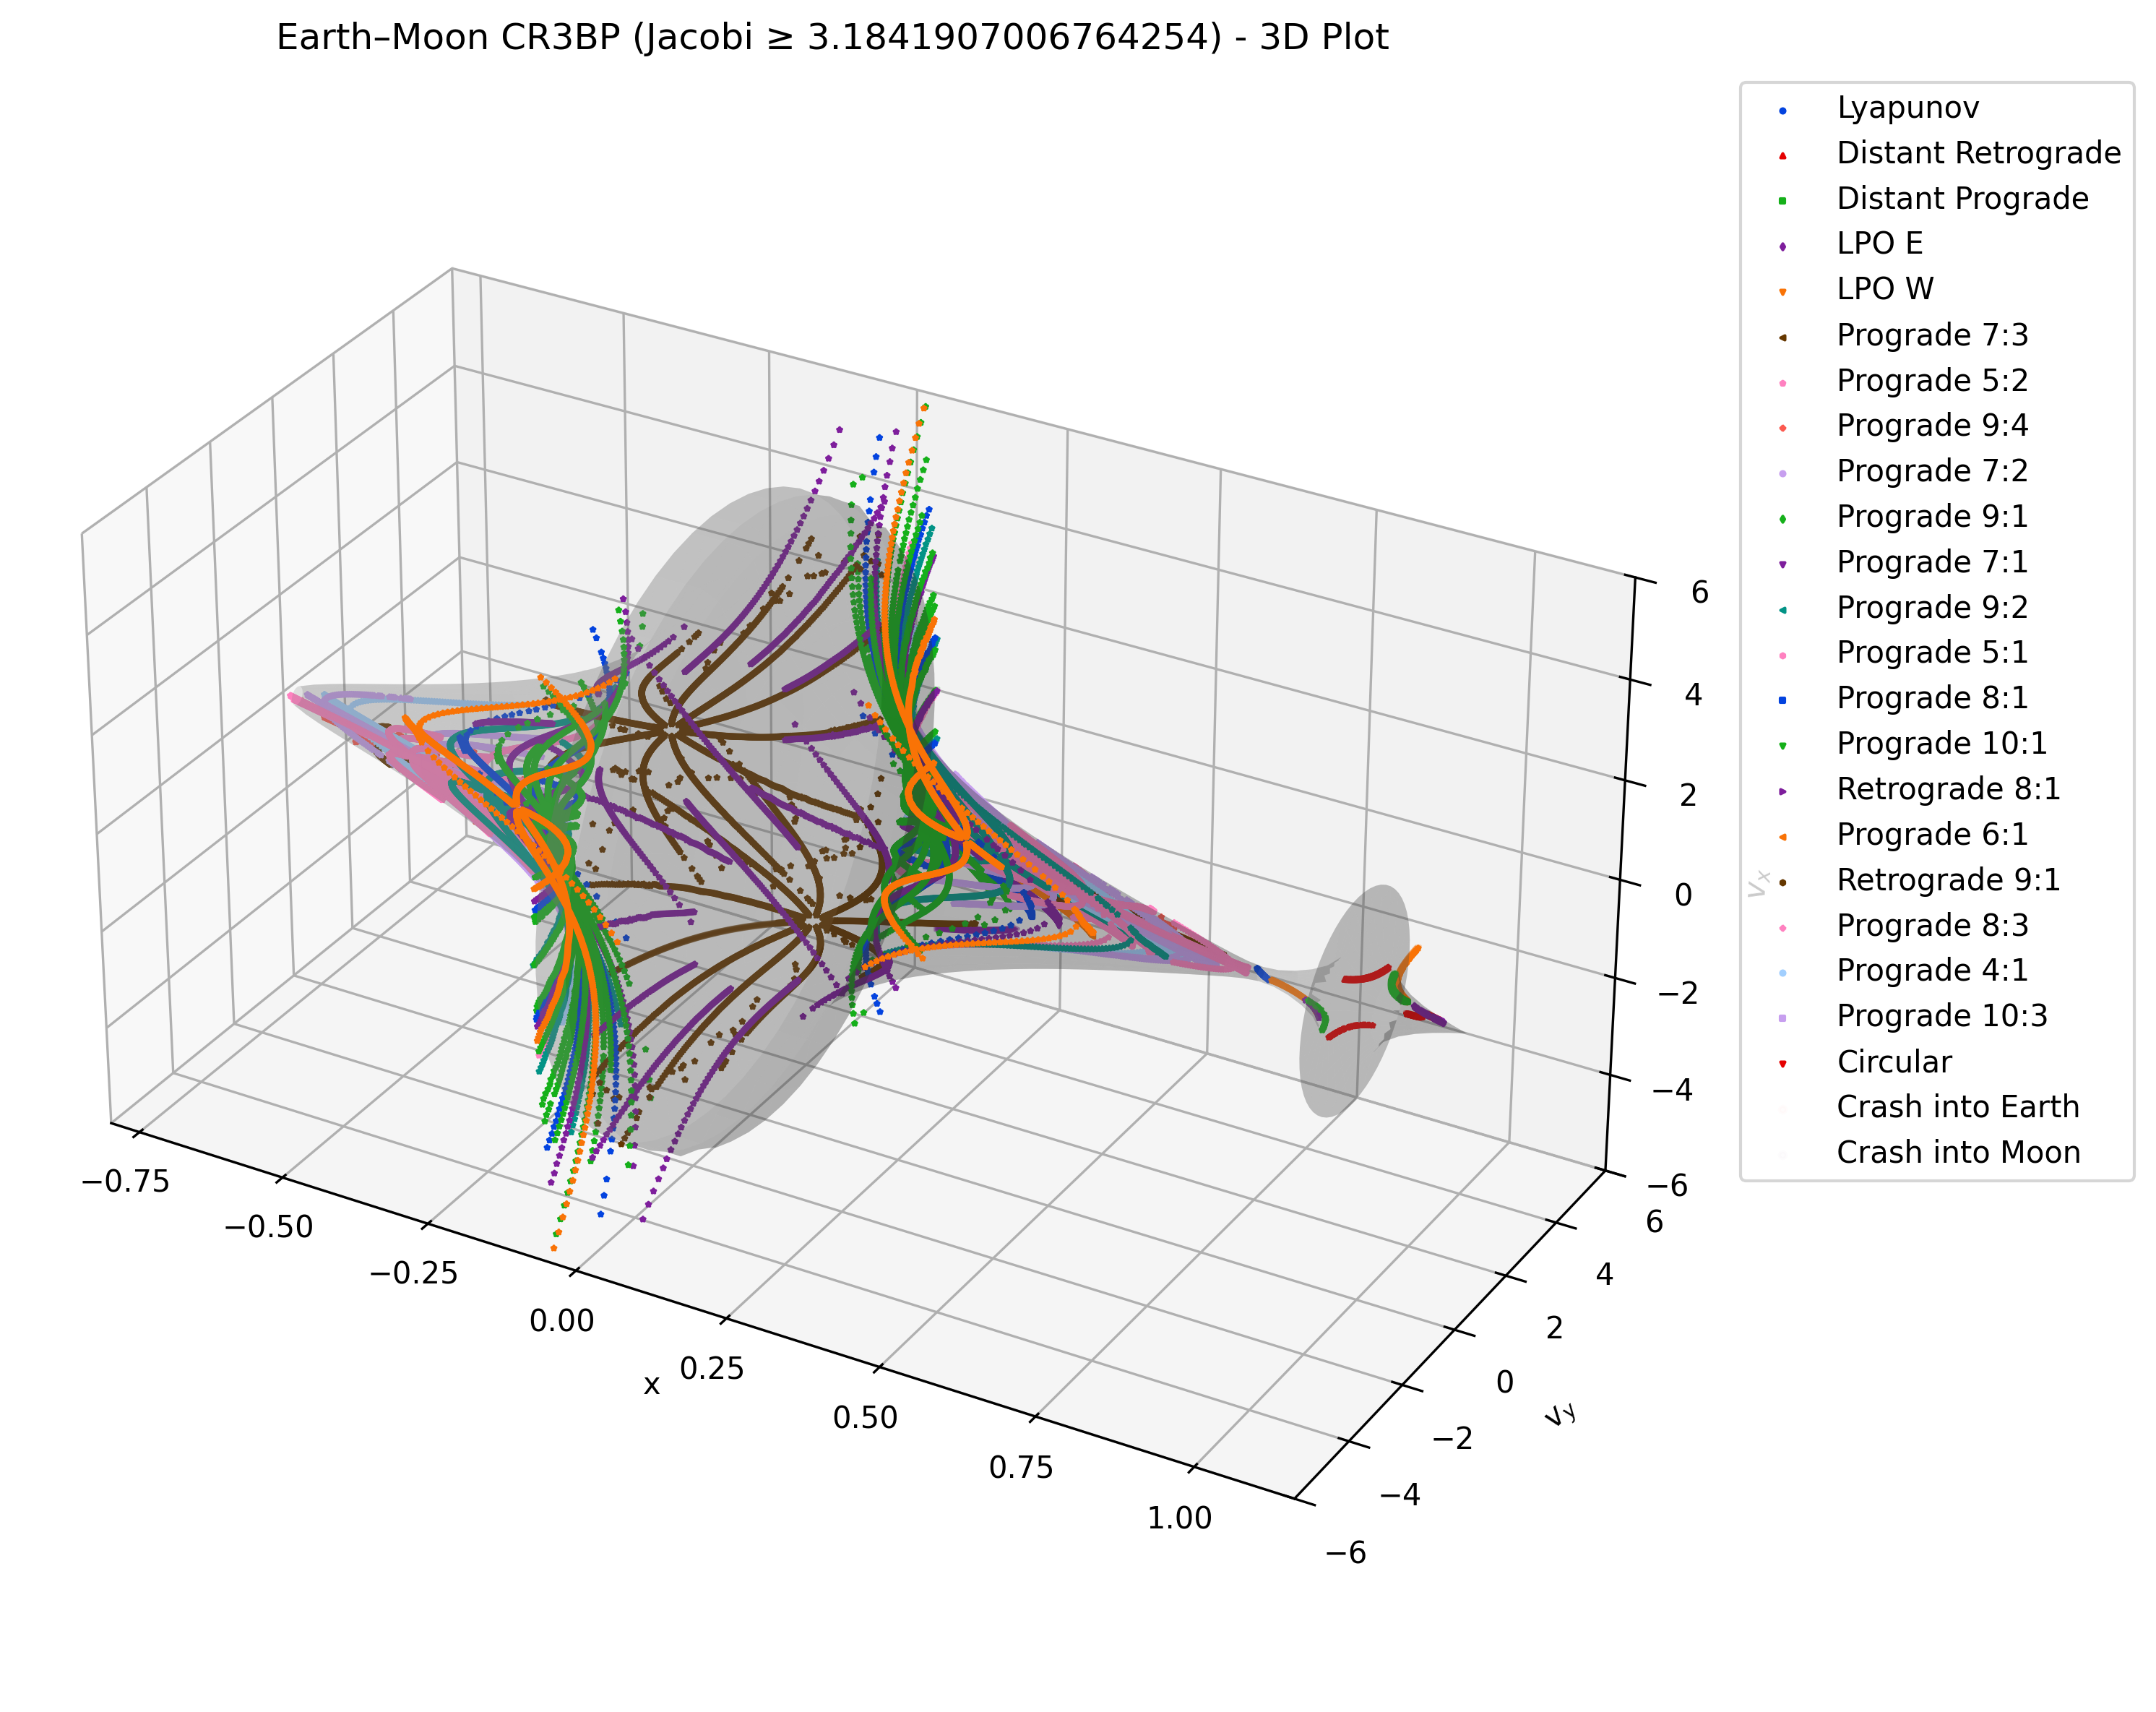
\includegraphics[width=2.9in]{images/3D crossings all orbits.png}
    % %     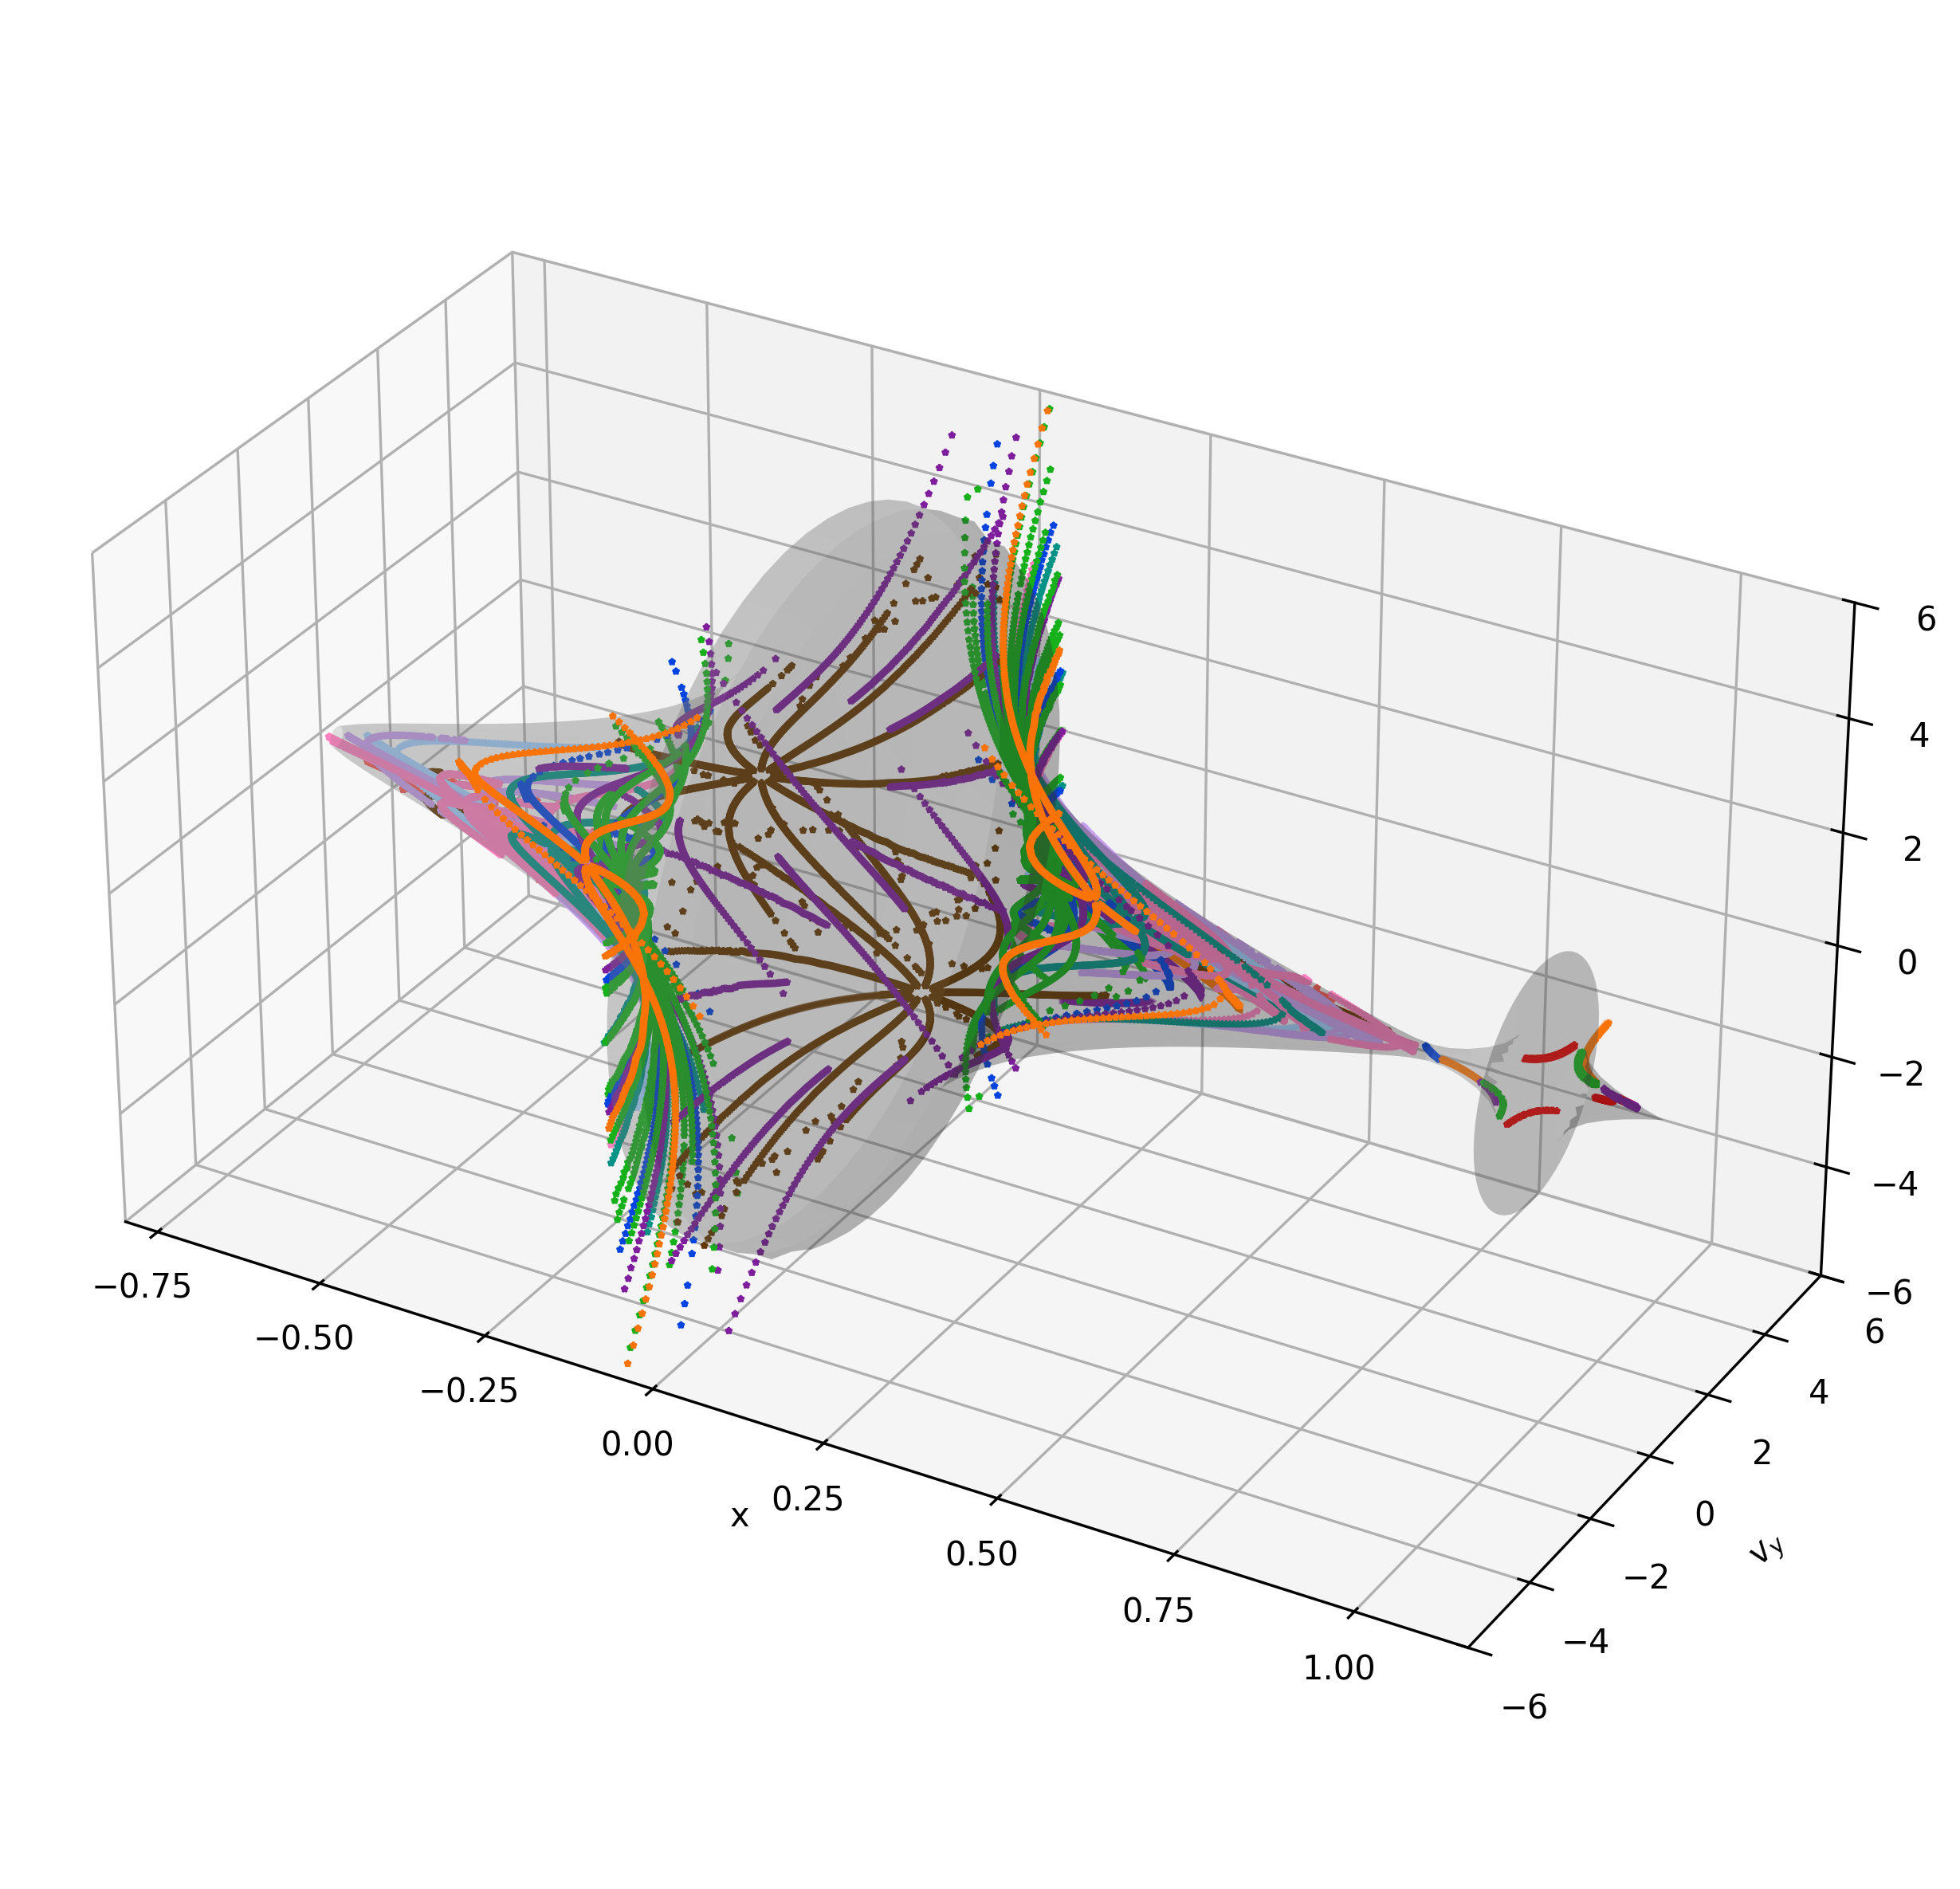
\includegraphics[width=2.9in]{images/3D crossings all orbits (without title and legend).png}
    % %     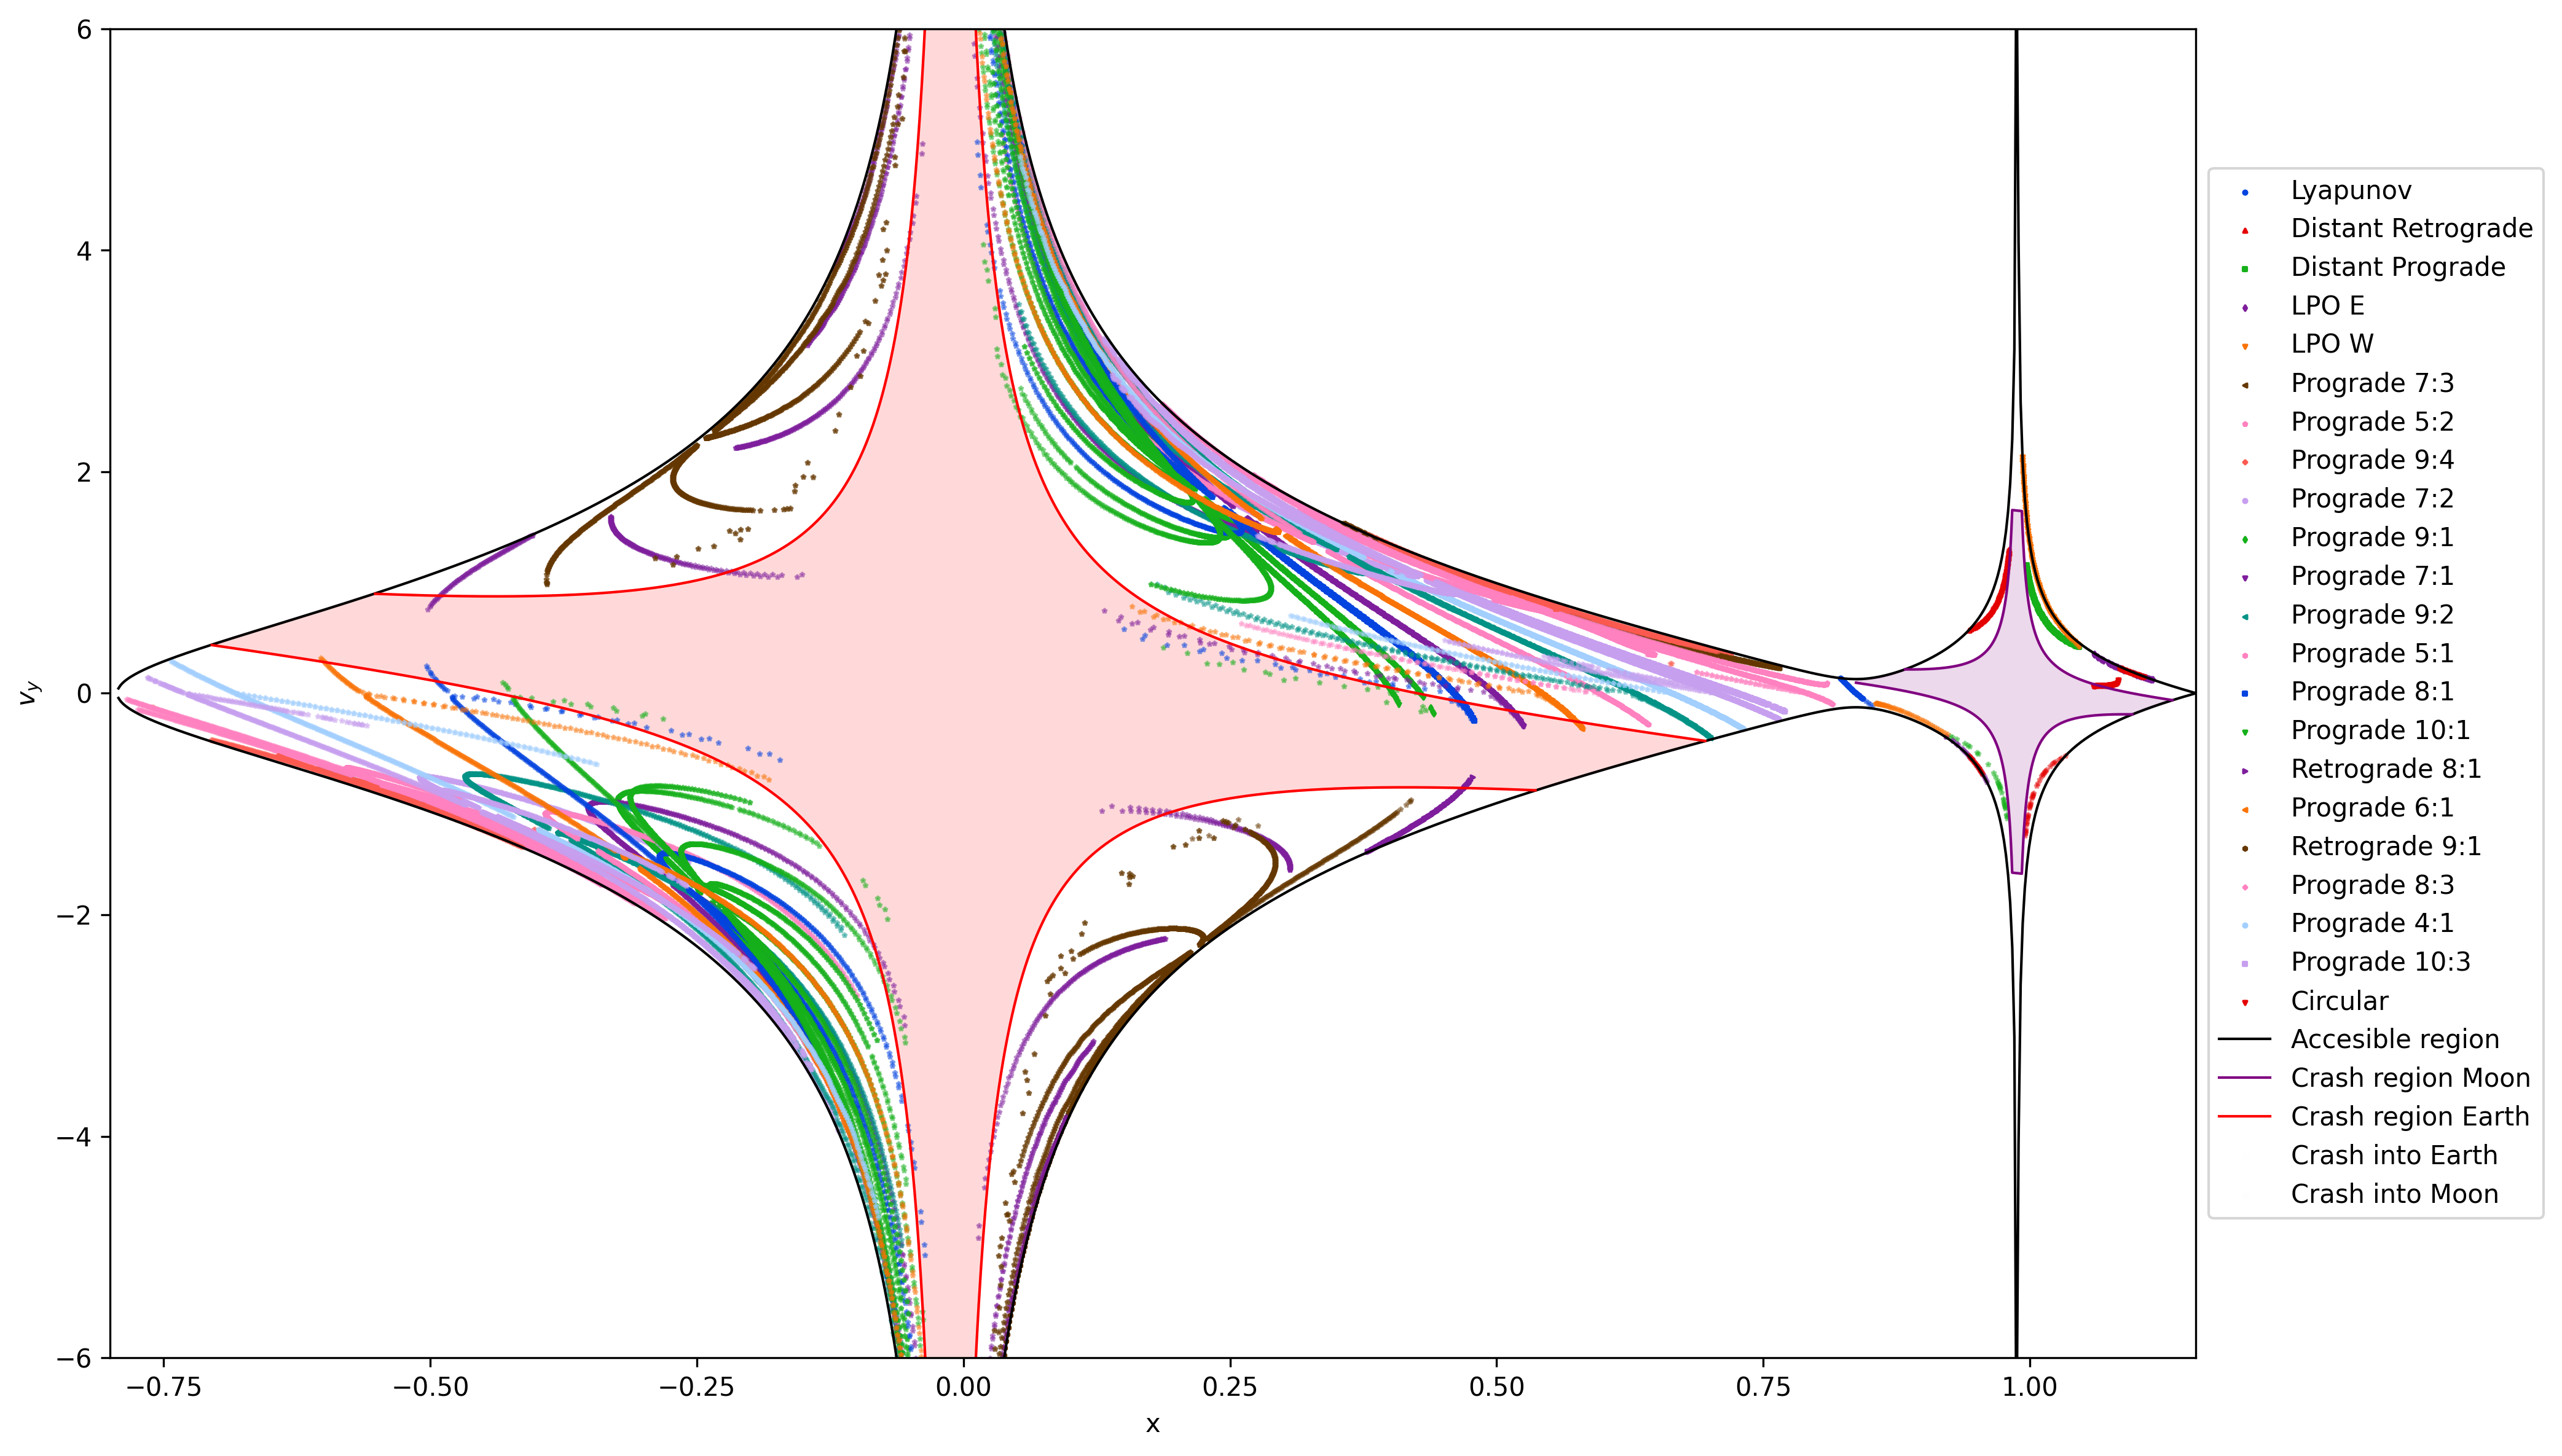
\includegraphics[width=in]{images/2D crossings all orbits.png}
    % %     \caption{Visualisations of the accessible region in three dimensions and its projection to the $(x,v_y)$ plane, displaying the Earth and Moon crash regions.}
    % % 	\label{fig:accesible region 3D and 2D}
    % % \end{figure}

    
    % \begin{figure}[htb] \label{fig:orbital crossings plotted}
    % 	\centering
    %     % 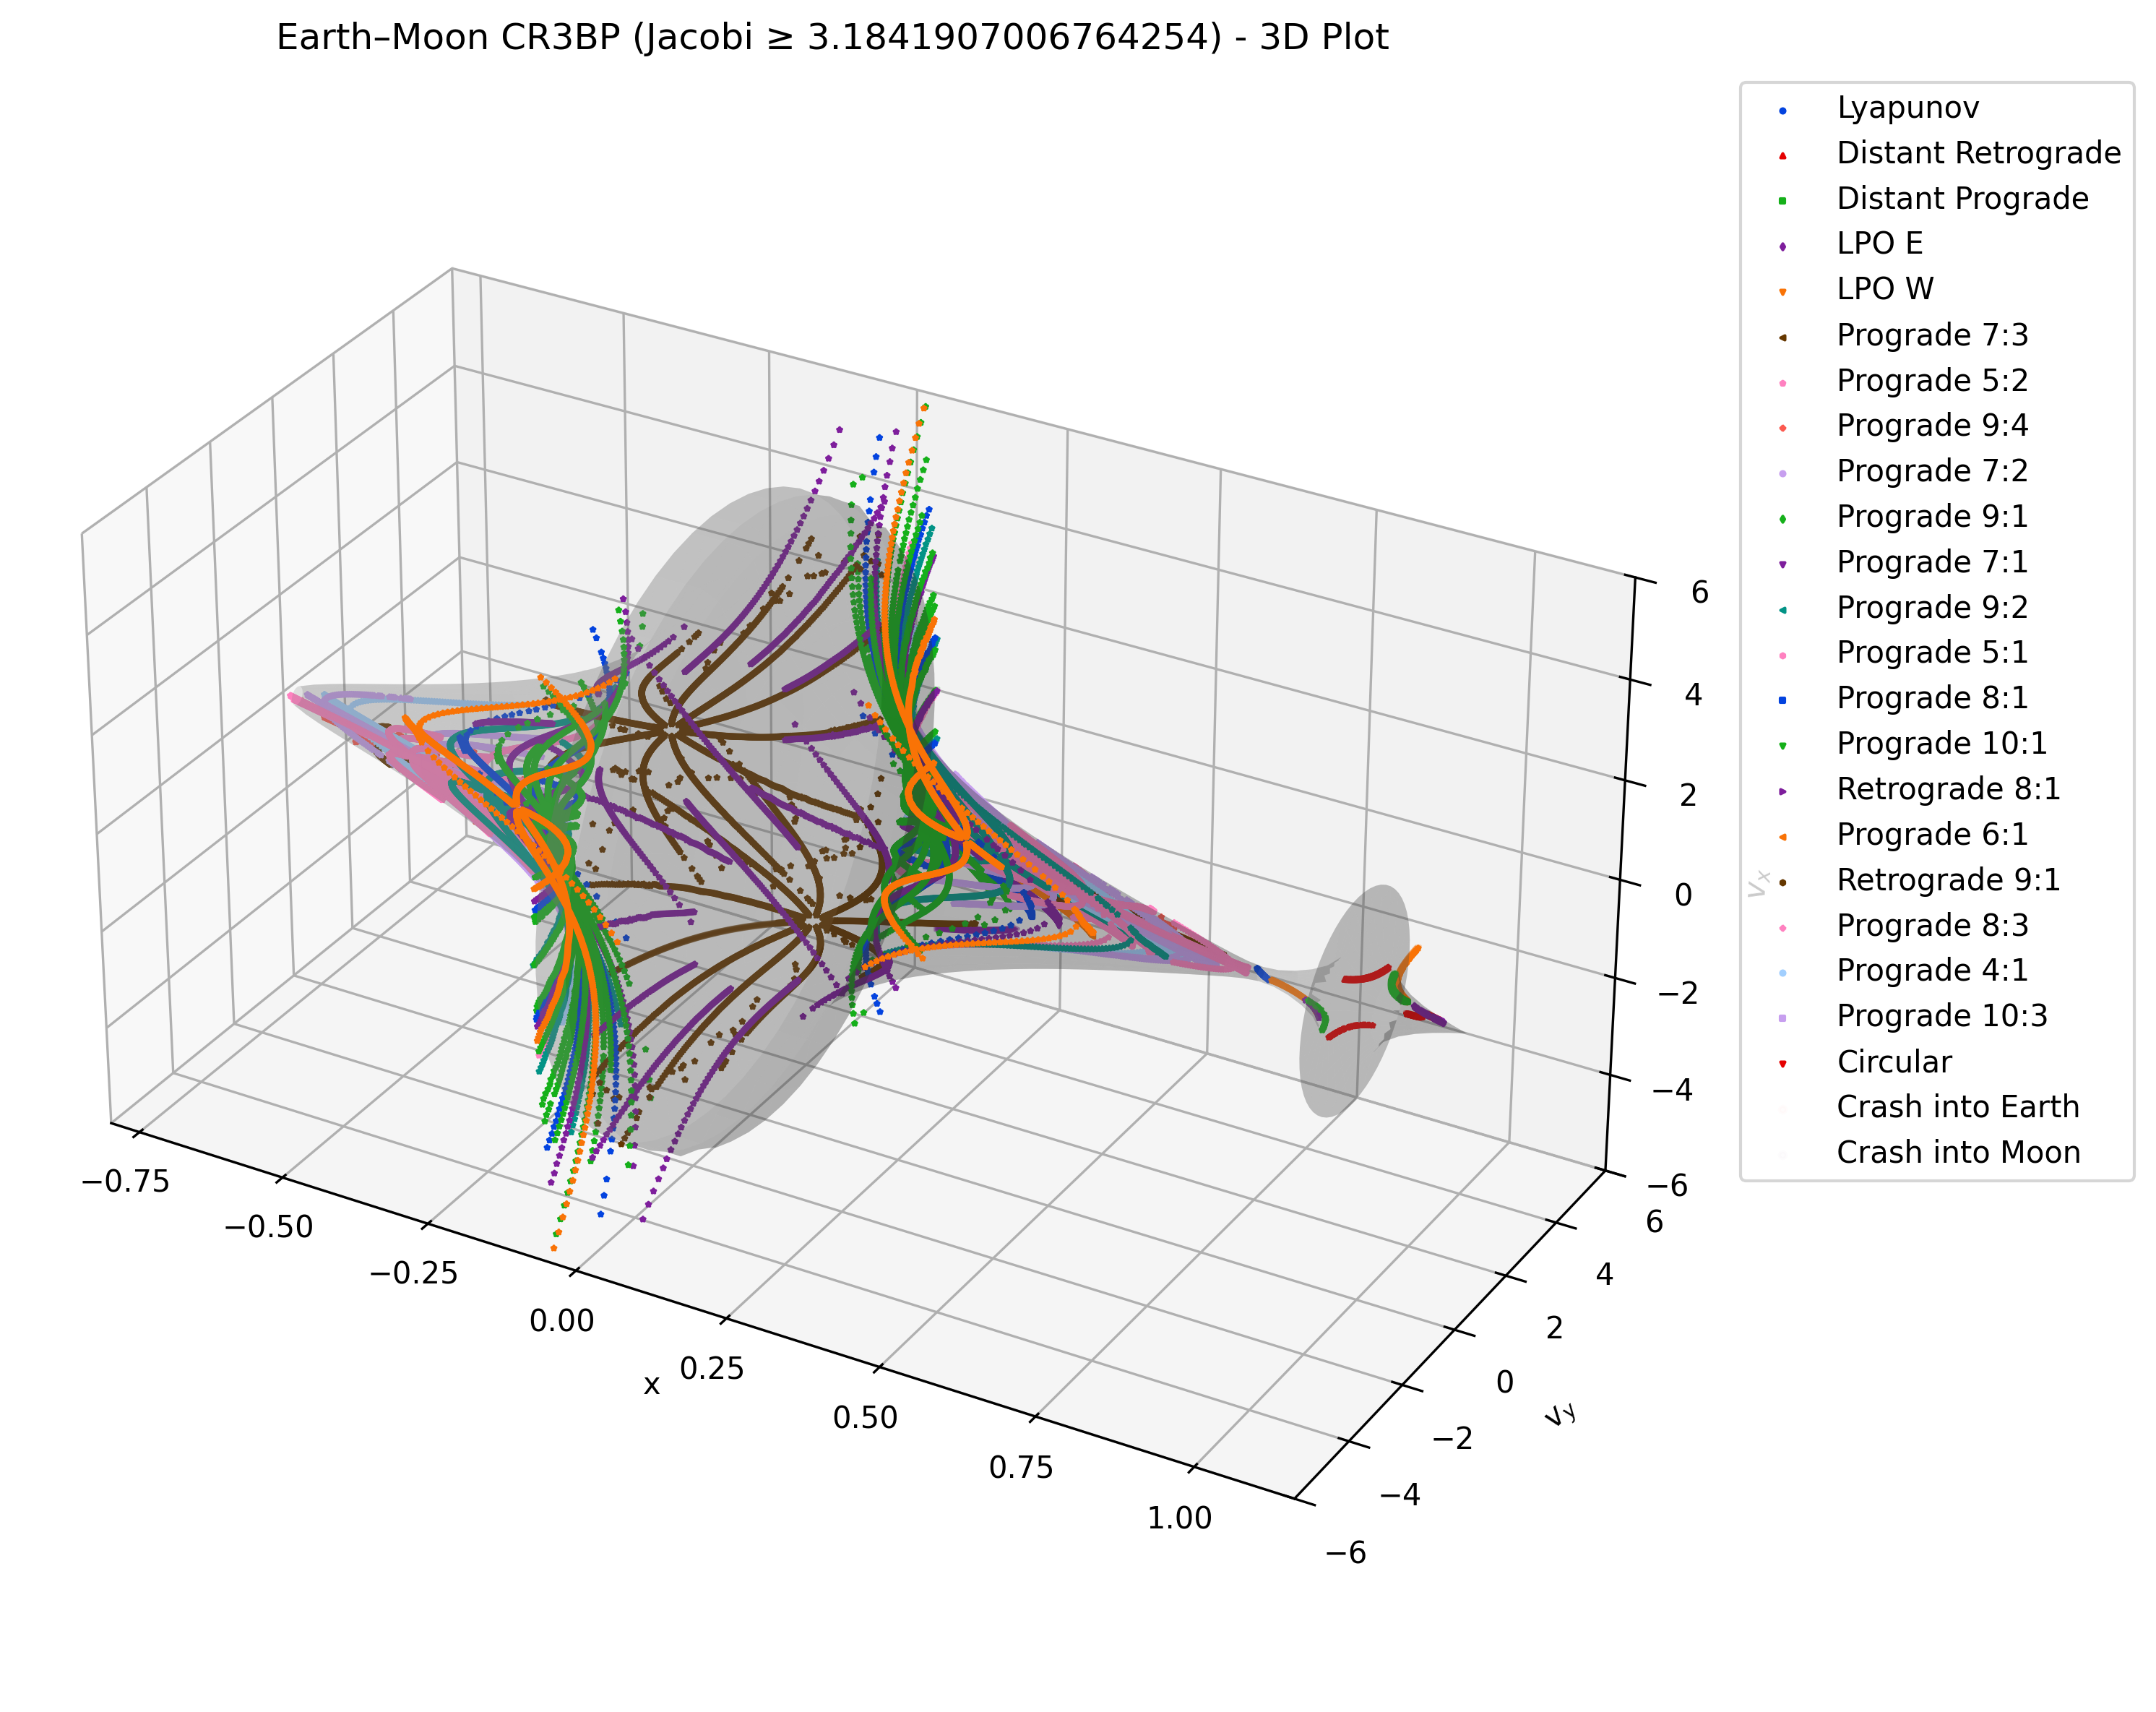
\includegraphics[width=2.9in]{images/3D crossings all orbits.png}
    %     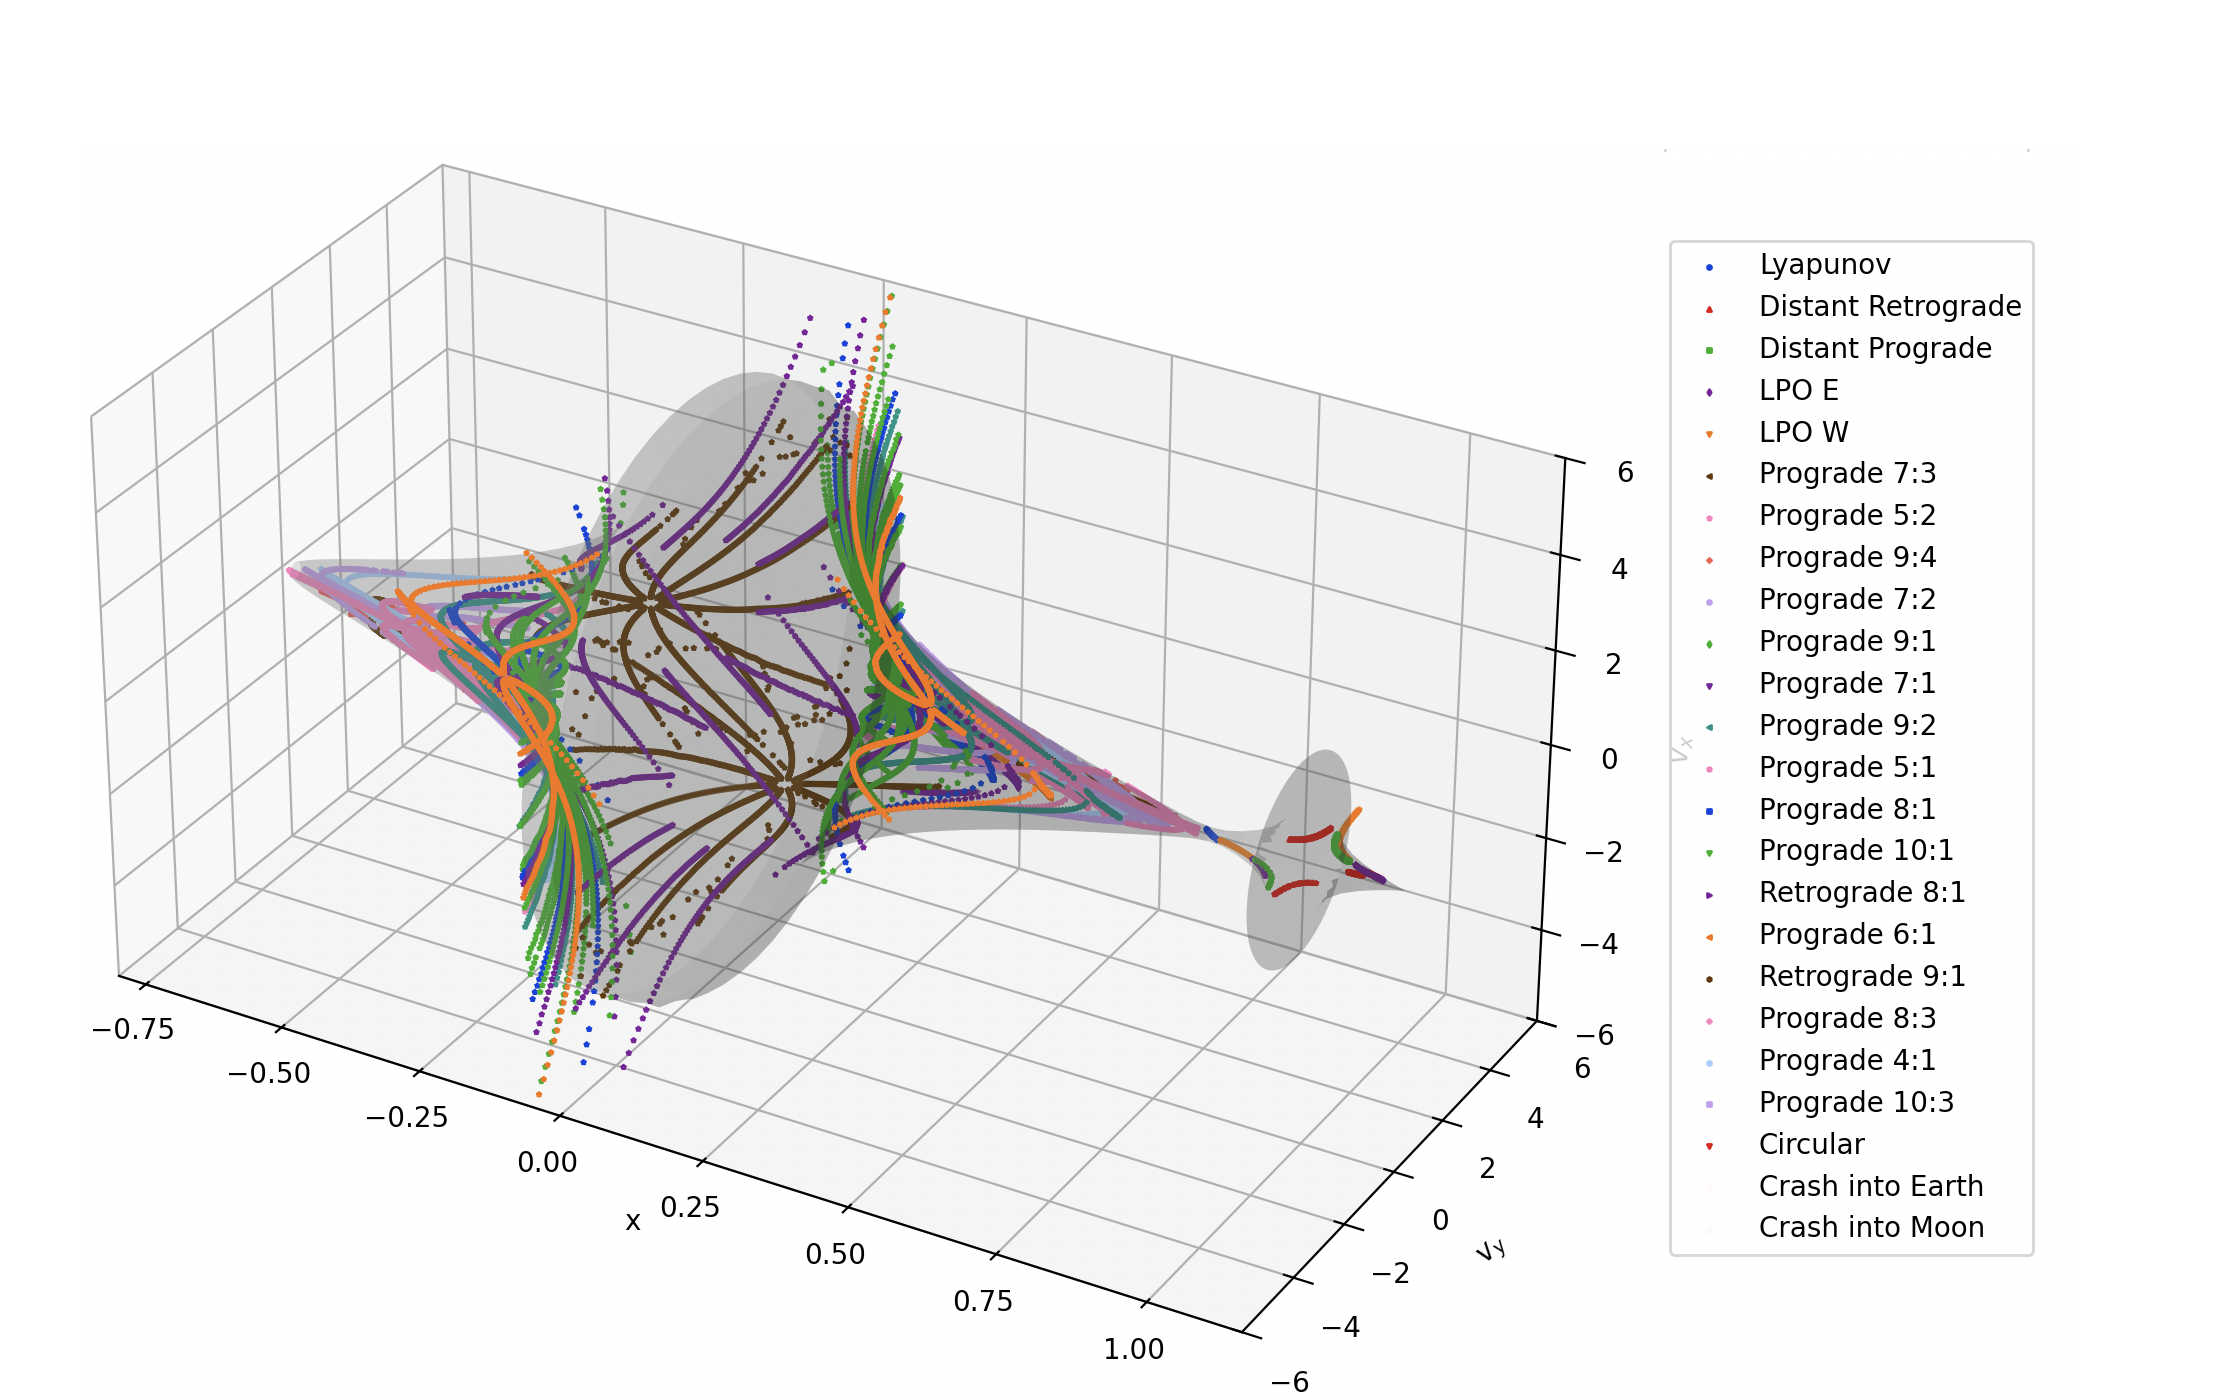
\includegraphics[width=0.85\linewidth]{images/manually made 3d.png}
    %     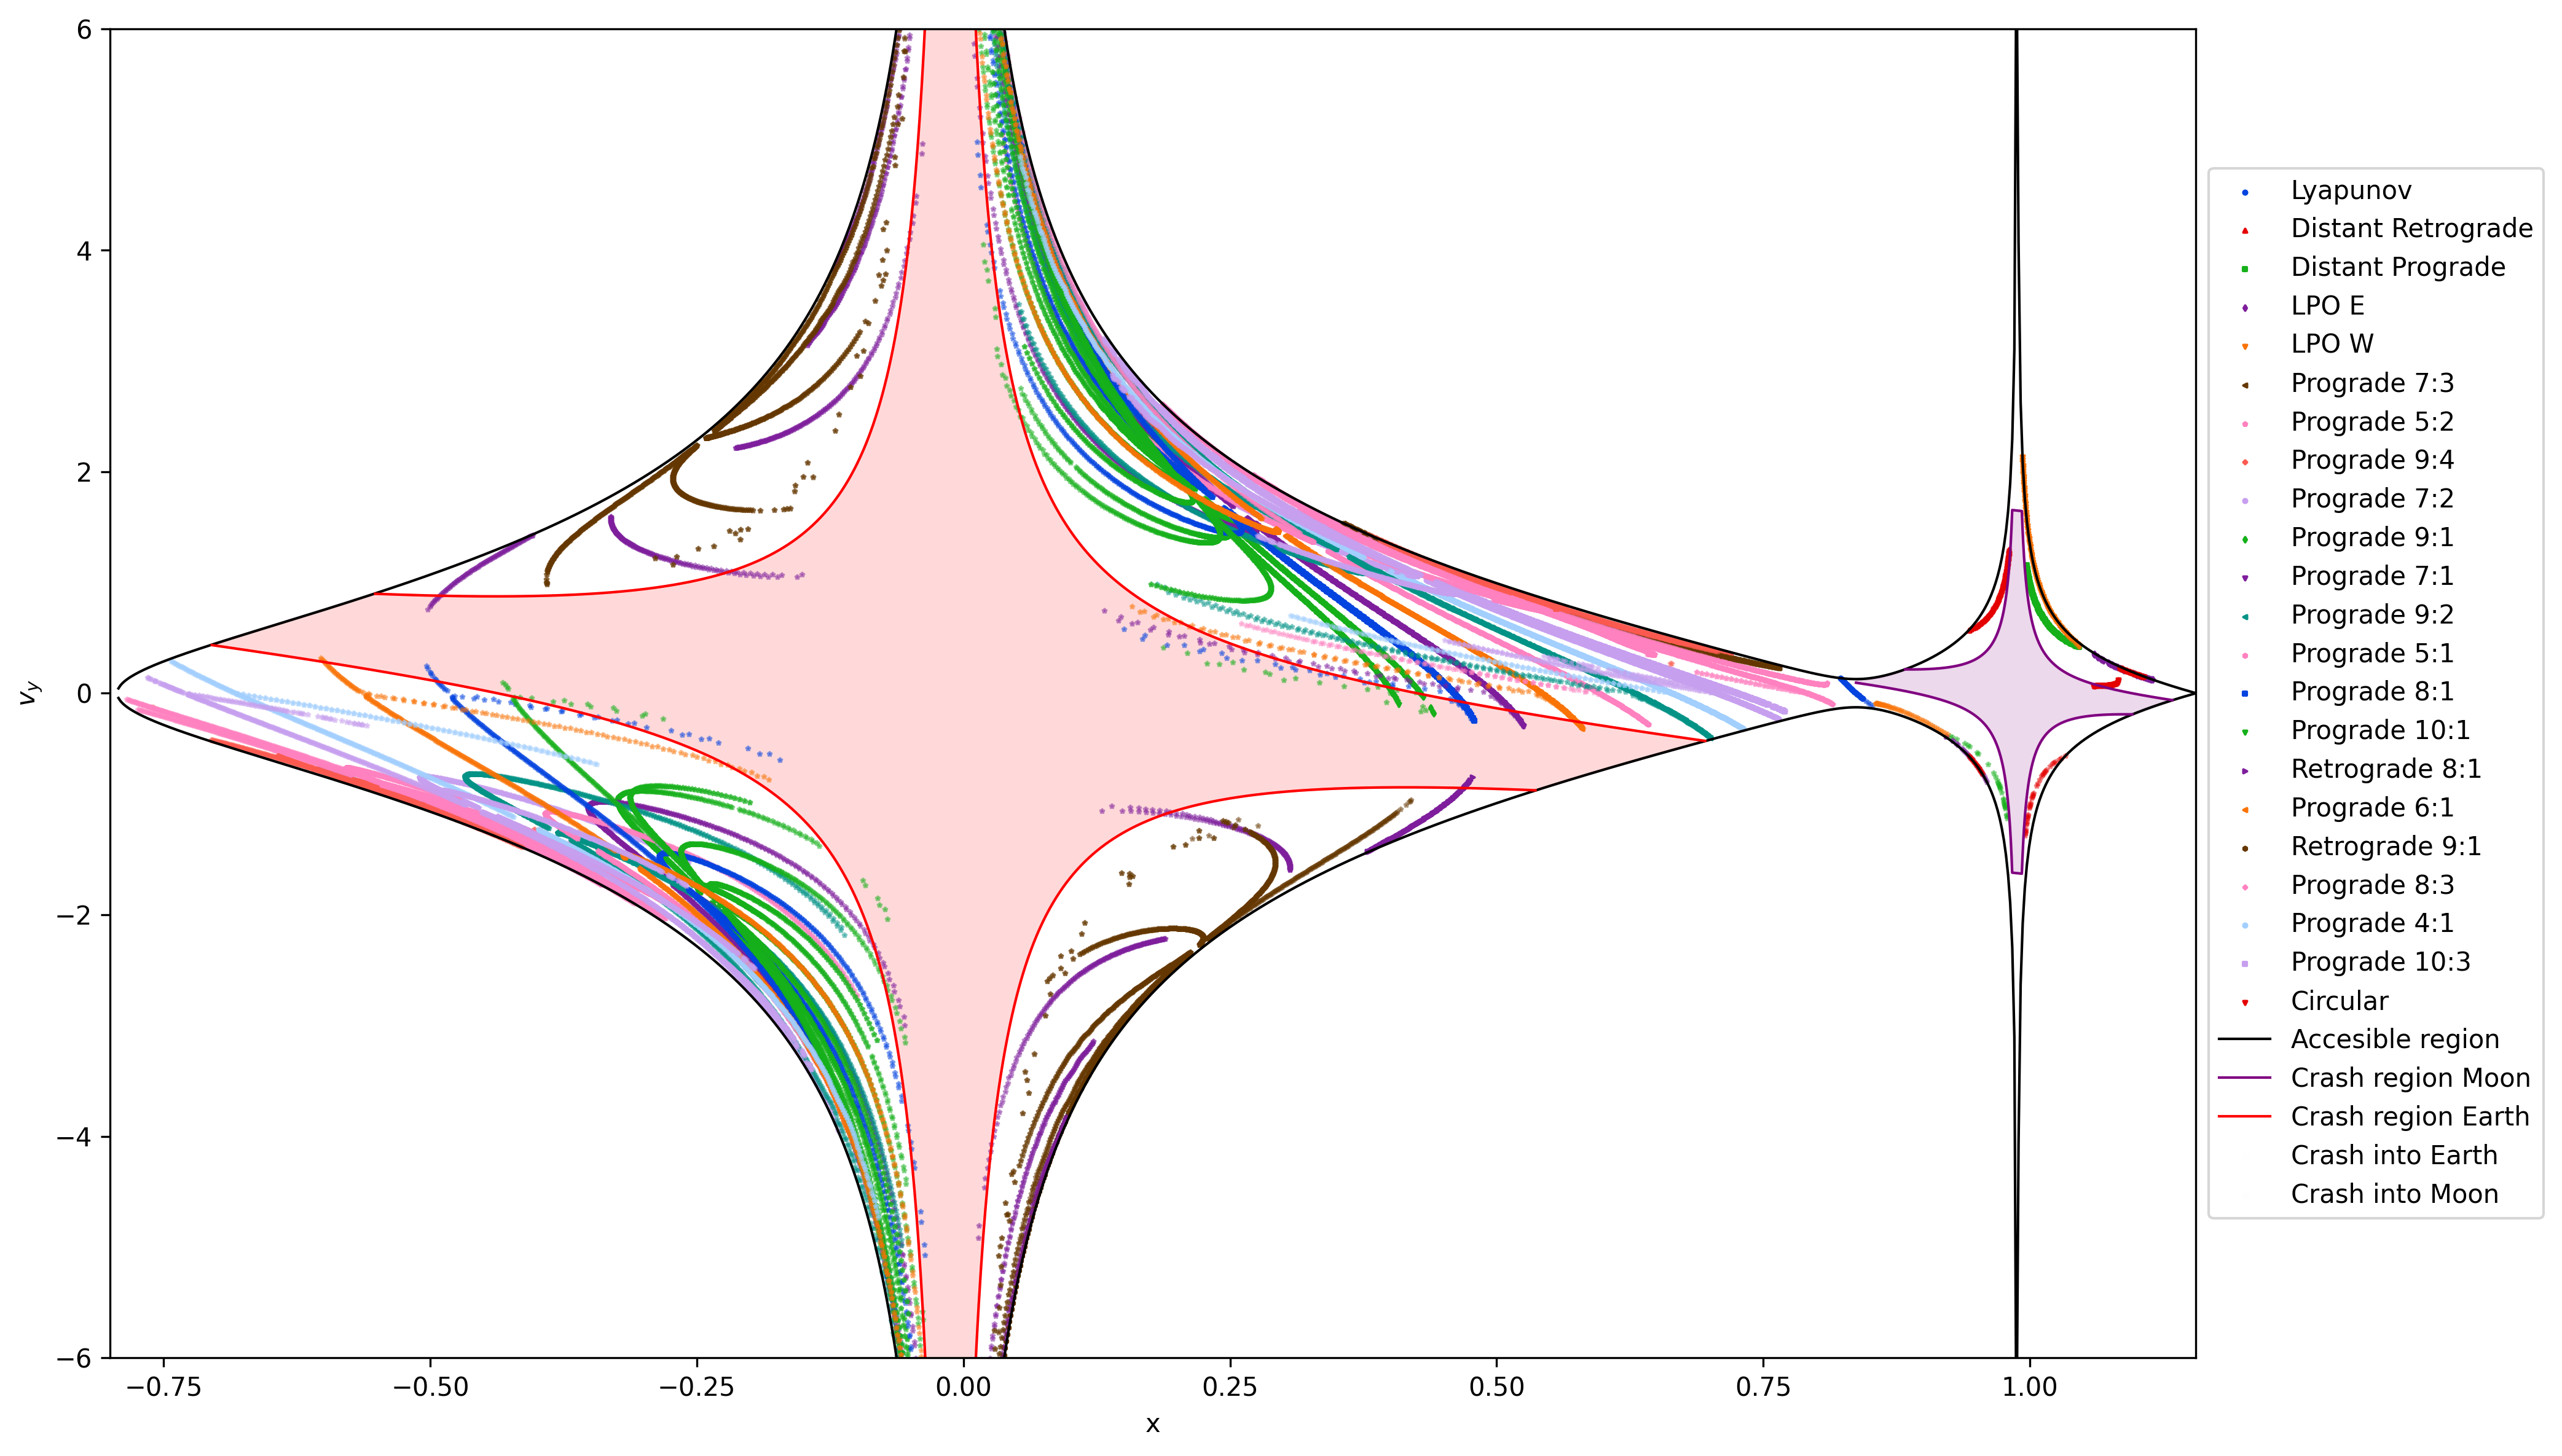
\includegraphics[width=0.75\linewidth]{images/2D crossings all orbits.png}
    %     \caption{Visualisations of the accessible region in three dimensions and its projection to the $(x,v_y)$ plane, displaying the Earth and Moon crash regions. The larger `pseudosphere'-esque region corresponds to the region around Earth, and the smaller: that of the Moon.}
    % \end{figure}



    % % \begin{figure}[htb]
    % %     \centering
    % %     \parbox[c]{2.9in}{%
    % %         % \centering
    % %         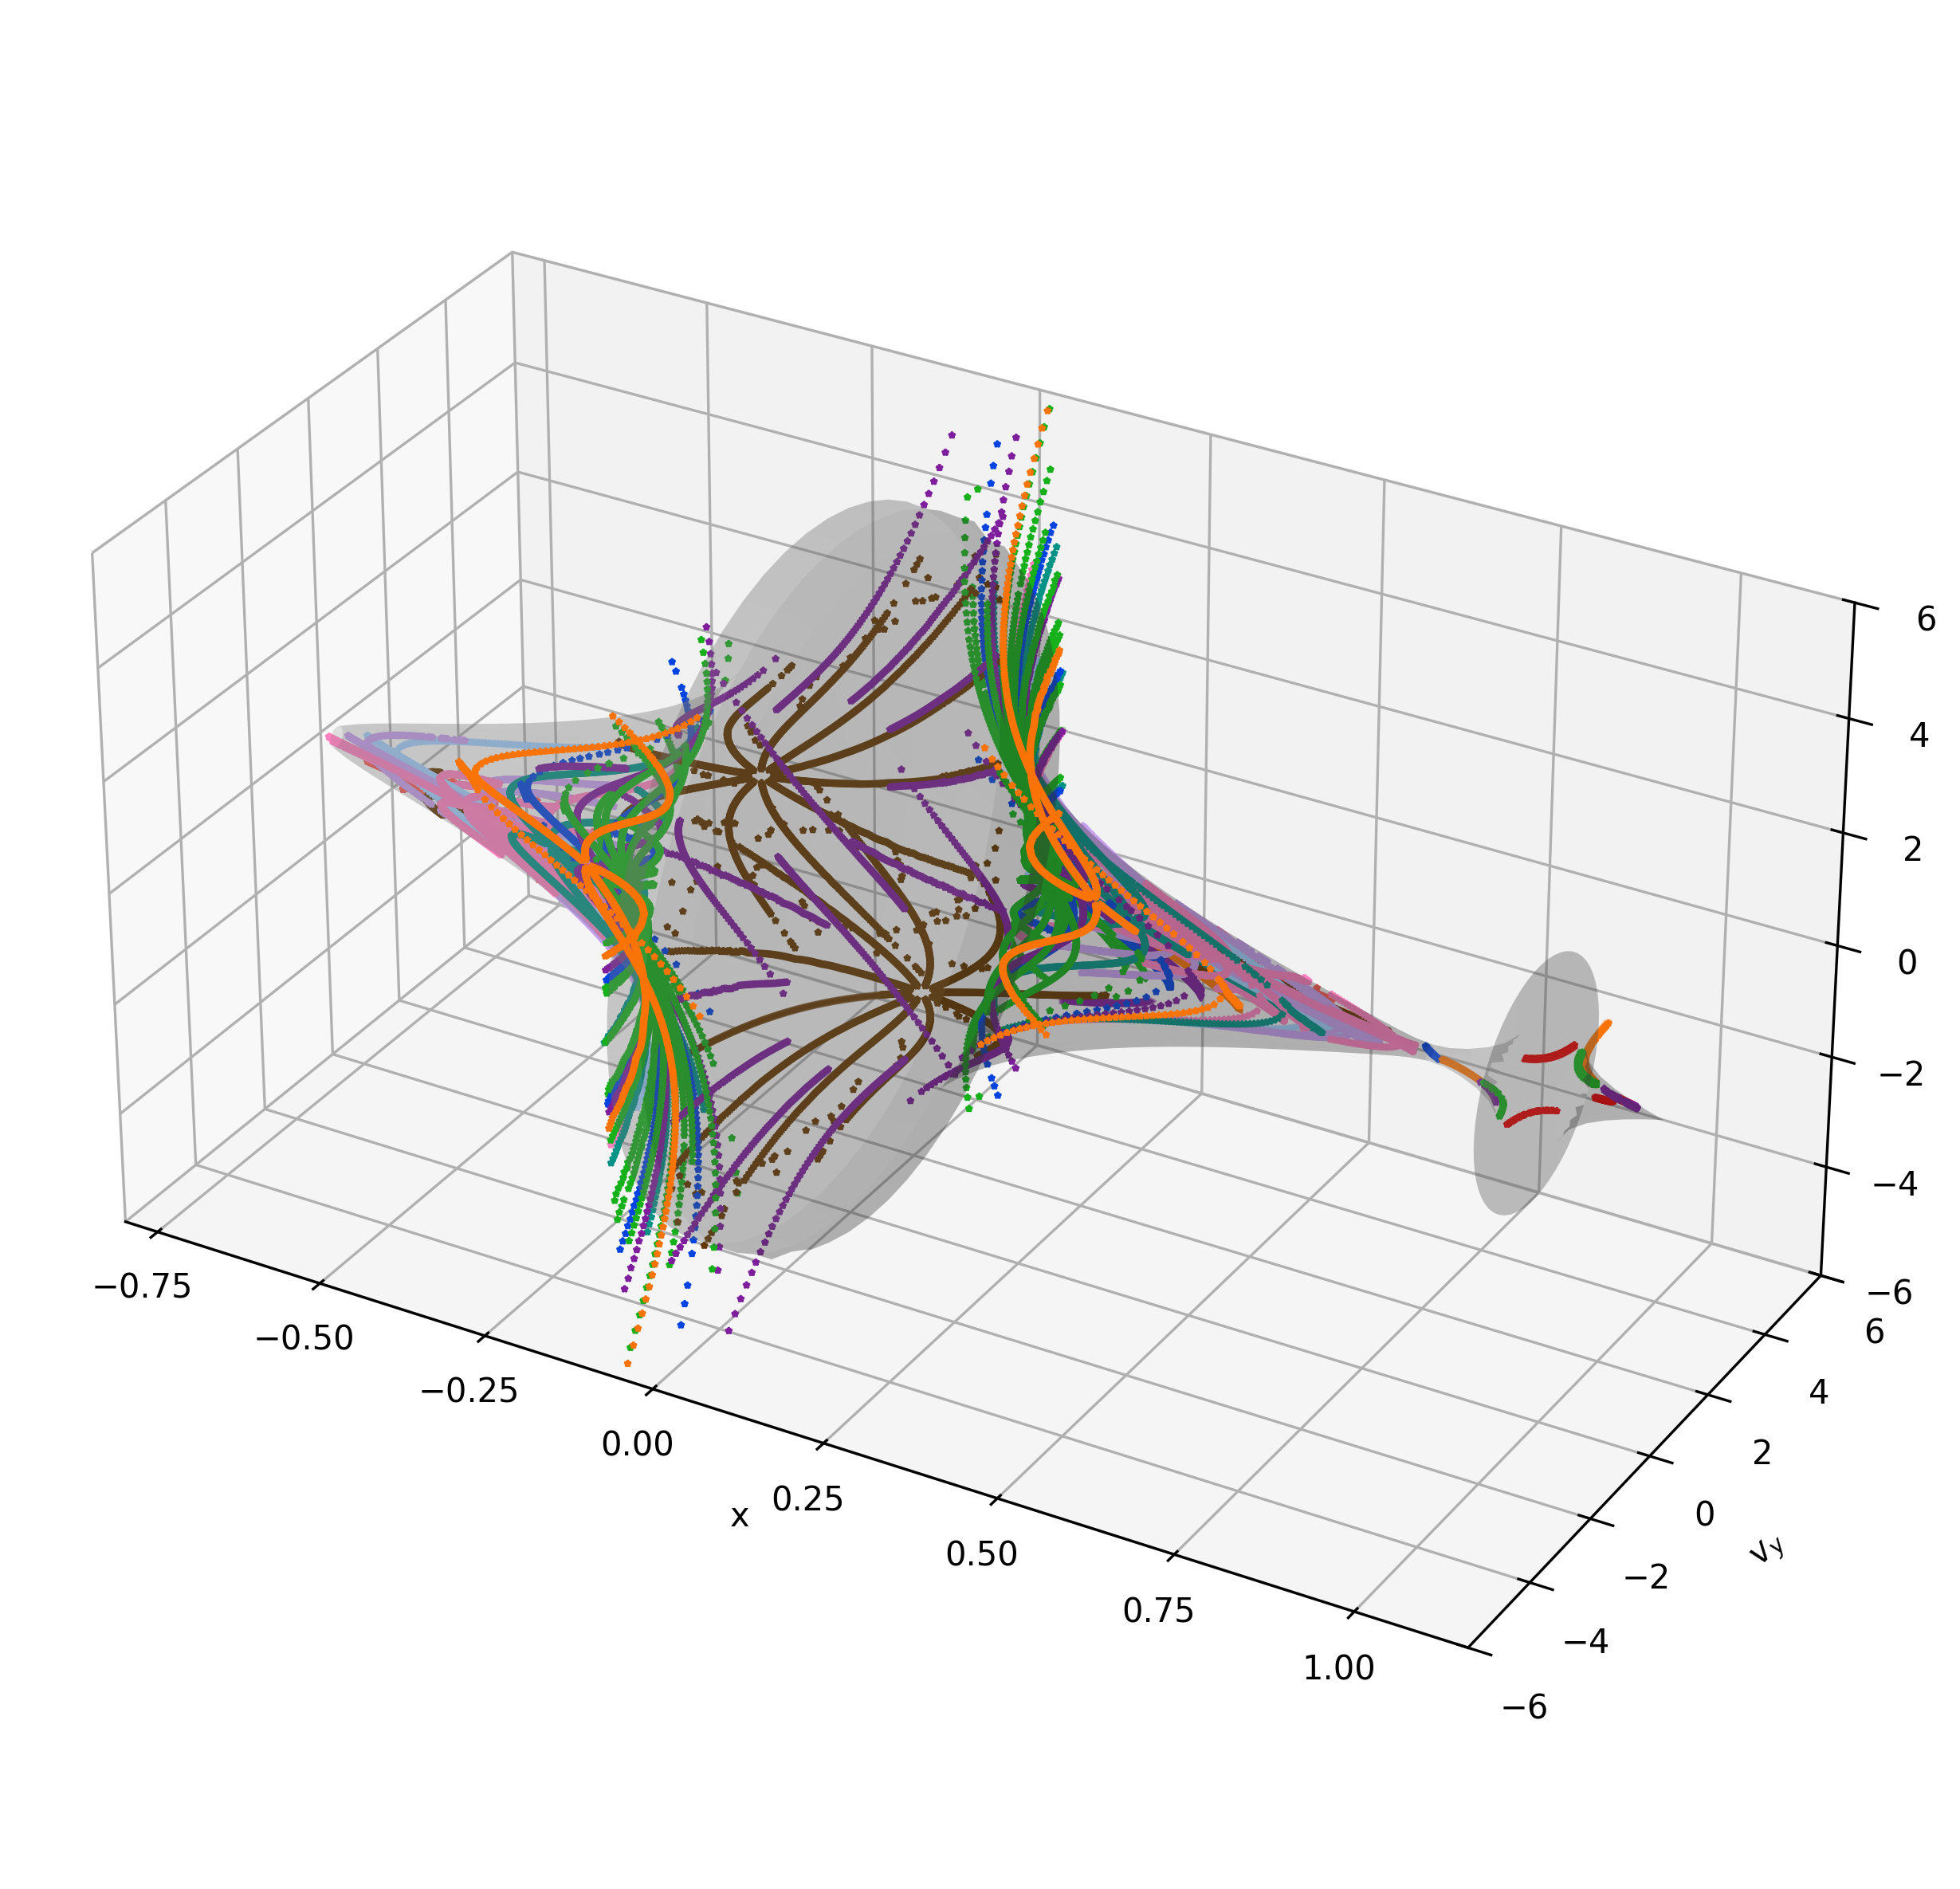
\includegraphics[width=2.9in, trim={1cm 0 0 0}, clip]{images/3D crossings all orbits (without title and legend).png}%
    % %     }%
    % %     % \hfill
    % %     \parbox[c]{3in}{%
    % %         % \centering
    % %         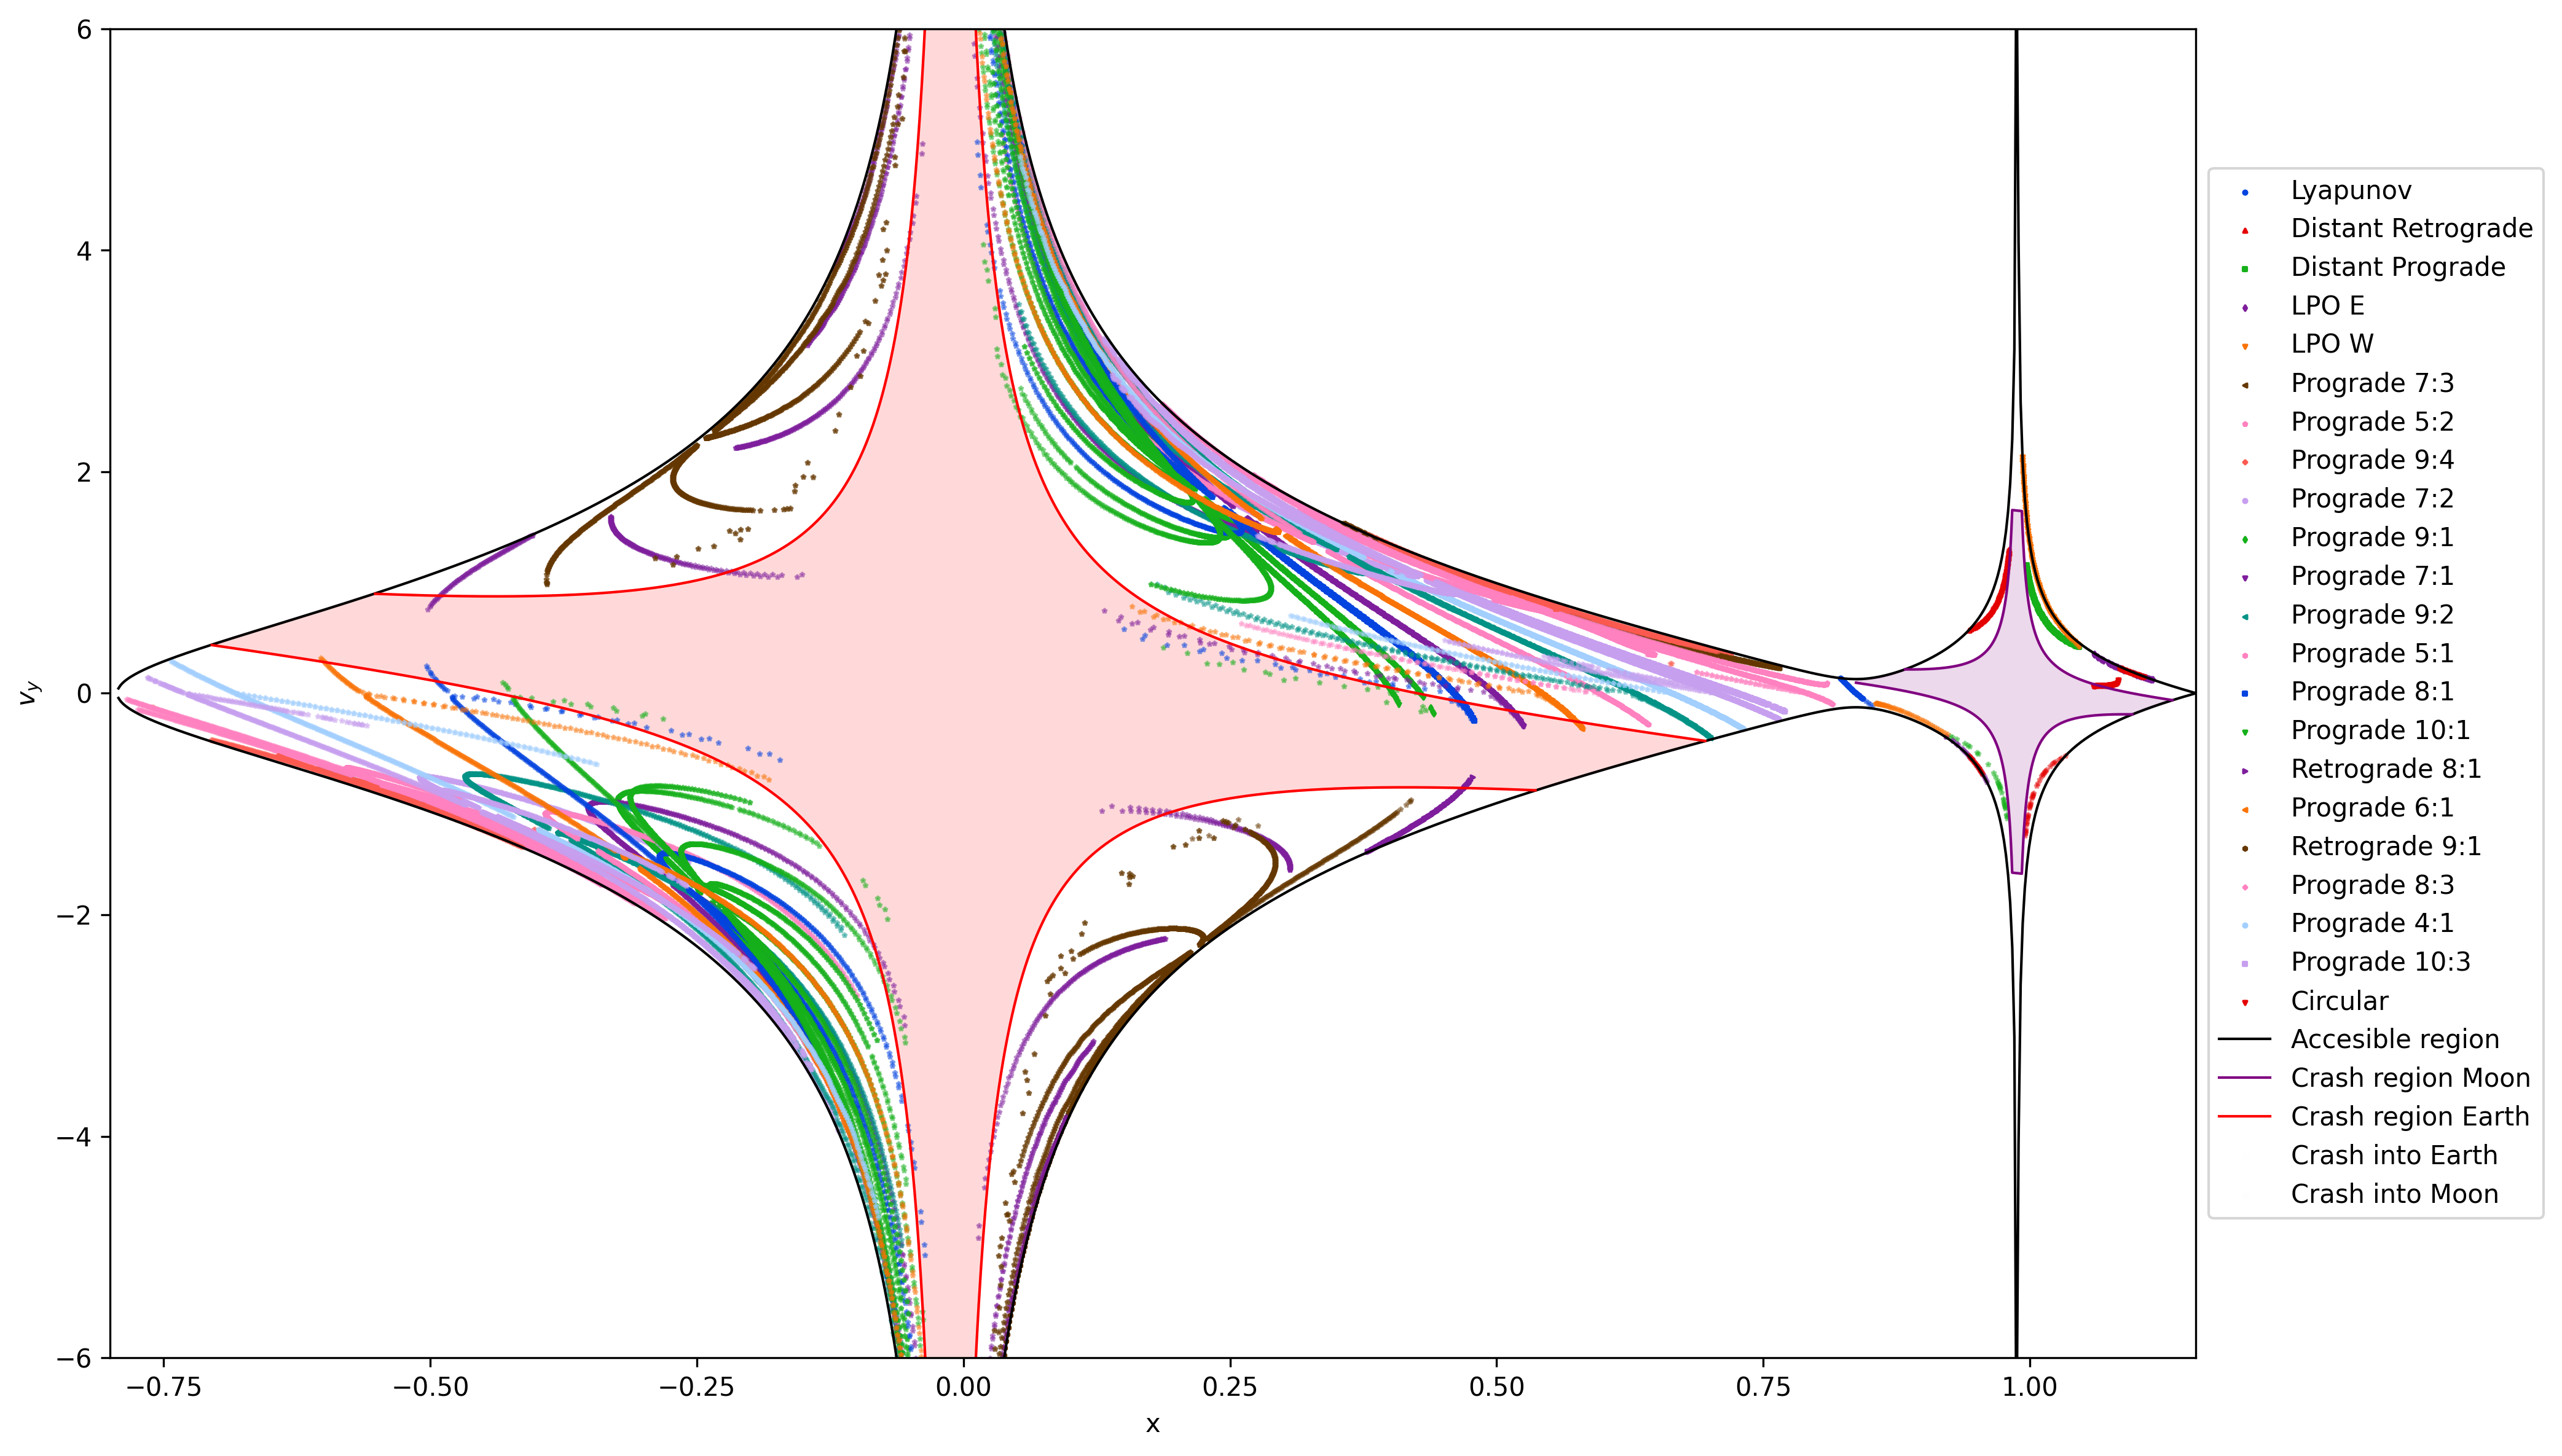
\includegraphics[width=3.5in, trim={0.3cm 0 0 0}, clip]{images/2D crossings all orbits.png}%
    % %     }
    % %     \caption{Visualisations of the accessible region in three dimensions and its projection to the $(x,v_y)$ plane, displaying the Earth and Moon crash regions.}
    % %     \label{fig:accesible region 3D and 2D}
    % % \end{figure}
        